%%% KCSS Dissertation Template
%%%
%%% Take care of all fields marked <++FOO++>.
%%% When using Vim LaTeX Suite <http://vim-latex.sourceforge.net/>,
%%% then Ctrl-j should navigate to the next such field.

\documentclass[10pt]{book}
\usepackage[language=english,theorems=numbersfirst,paper=a4paper]{ifiseries}
\usepackage{listings}
\usepackage[ruled,vlined]{algorithm2e}
\usepackage{pdfpages}
\usepackage{todonotes}
\usepackage{breakurl}
\usepackage{subcaption}
\usepackage{hyperref}
\usepackage{lipsum}
\usepackage{parcolumns}
\usepackage[printonlyused]{acronym}
\usepackage{bm,amsmath}
\usepackage[newfloat]{minted}
\usepackage{caption}
%\usepackage{mathtools}
\setlength{\marginparwidth}{3cm}
\addbibresource{thesis.bib}

\graphicspath{{./assets/}}

\newenvironment{localsize}[1]
{%
  \clearpage
  \let\orignewcommand\newcommand
  \let\newcommand\renewcommand
  \makeatletter
  \input{bk#1.clo}%
  \makeatother
  \let\newcommand\orignewcommand
}
{%
  \clearpage
}
% Minted env
\newenvironment{code}{\captionsetup{type=listing}}{}
\SetupFloatingEnvironment{listing}{name=Pseudocode}

\newcommand{\figureref}[1]{\textbf{\autoref{#1}}}
\newcommand{\figurereft}[2]{\textbf{\autoref{#1} #2}}
\newcommand{\toxdo}[1]{}

\newcommand*\NewPage{\newpage\null\thispagestyle{empty}\newpage}

\begin{document}

\frontmatter

\studtitlepage%
{ArUco Marker Detection on Flexible Photonic Crystals}%
{}
{Niklas Carstensen}%
{Master's Thesis}%
{\today}%
{Prof. Dr. Reinhard Koch}%
{Jakob Nazarenus, Tim Michels}%
\NewPage{}
\setcounter{page}{2}
\studeidesstatt
\NewPage{}

\selectlanguage{english}
\setcounter{page}{3}
\chapter*{Abstract}
TODO

\tableofcontents
\listoffigures
%\listoftodos
\mainmatter
\chapter{Introduction}

The world faces a shortage of health workers, that is projected to endure into 2030 \cite{BMJHealthWorkforce22}, while 47\% of available health workers cared for 22\% of the worlds population in 2020. This shortage and unequal distribution of health workers drive the need for more efficient care for patients. 

A part of the solution for this problem could be small and inexpensive testing equipment \cite{Fab23}, which would allow for fast and regular assessment of ones health without requiring the time of healthcare professionals \cite{POC12}. Such an approach is called \ac{POC}, since the testing and evaluation is done by and of the patient. These kits are also called \acp{POCT}. One type of \ac{POCT} are wearables. However traditional wearables are based on electrical readout systems \cite{gao2019flexible}, which necessitate conducting wires and a battery and may be invasive. To overcome the drawbacks of wearables using electrical readout systems, optical readout systems can be used instead \cite{nguyen2021wearable}. One approach for an optical readout system is using commercially available adhesive tape, which acts as a \ac{PCS}, and etching \ac{ArUco} fiducial markers into it \cite{Fab23}. This is done by first applying a negative photoresist to the tape and then shining UV light on it, while masking the parts of it that are supposed to become part of the \ac{ArUco} shape later. Then an \ac{IBE} process is applied to the tape and finally the heat resist of the first step is removed during an ultrasonic heat bath.

\section{Problem Statement}

This work focuses on the detection of the \ac{ArUco} fiducial markers, that were etched into tape, using neural networks. Since the tapes should be used as \acp{POCT} by patients, the technology developed here is supposed to run on patients smart phones. While smart phones are easily carryable, they come with the drawback of not having much space or energy for large \acp{GPU}, which limits the choice of models.

% TODO: Explain difficulty with example iamges

\section{Outline}

TODO

\chapter{Preliminaries}
\label{chap:prelim}

The later chapters of this thesis are based on a number of technologies and concepts, which is why important definitions and terms are explained here.

\section{Definitions}

The term dataset\footnote{\url{https://en.wikipedia.org/wiki/Data_set}, accessed on 01.10.2023} is central to machine learning as it defines what is learned from. However this term is ambiguous as it describes both a series of images and labels\footnote{\url{https://pytorch.org/tutorials/beginner/introyt/trainingyt.html}, accessed on 01.10.2023} as well as a set of series of images and labels \cite{lin2014microsoft}. In other subfields of machine learning a dataset may contain different data types other than images. For this thesis however dataset and similar terms are defined as follows to make the later parts more easily understandable:

\begin{description}
  \item[Label] A \textit{label} or \textit{annotation} refers to extra data that belongs to an image and describes a subset of the images contents. \textit{Labels} are usually created using human input and describe the desired output of a machine learning model on that image.
  \item[Dataseries] A \textit{dataseries} refers to a series of images and labels
  \item[Dataset] A \textit{dataset} refers to a combination of usually up to three \textit{dataseries}.
  \item[Datagroup] A \textit{datagroup} refers to a \textit{dataseries} in the context of a \textit{dataset}. Typical \textit{datagroups} are 'training', 'validation' and 'testing' or 'train', 'val' and 'test' for short.
\end{description}

\section{Neural Networks}

This section gives a brief overview over \acp{ANN}. Since this thesis is written from a computer science perspective the term \acp{NN} is used interchangeably with \acp{ANN}.

\subsection{History}

Neural network interest and therefore research happened in waves over the last decades, starting with McCulloch and Pitts' work on logical operations on neurons in 1943 \cite{mcculloch1943logical,485891}. 

\begin{figure}
  \caption{Visualization of a perceptron}
  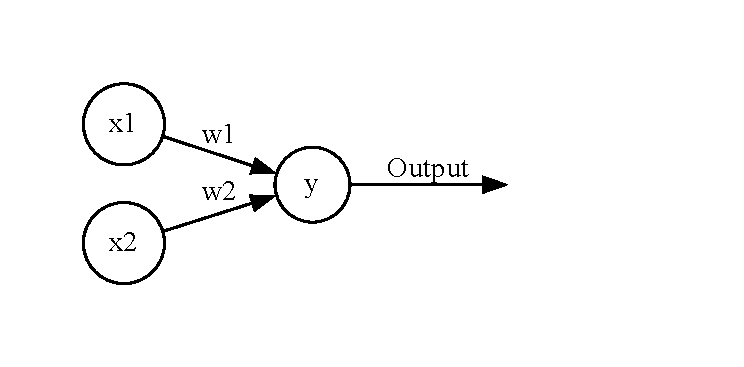
\includegraphics[width=0.5\textwidth]{graph/rosenblatt}
  \label{fig:perceptron}
\end{figure}

The second wave started in the early 1960ies with Rosenblatt's perceptron convergence theorem \cite{rosenblatt1962principles}. A visualization of the perceptron can be seen in \figureref{fig:perceptron} and the output of the perceptron is calculated as follows:
\[
    p(x)= 
\begin{cases}
    1, & \text{if } \sum_i w_ix_i + b > 0\\
    0, & \text{otherwise}
\end{cases}
\]
Setting $w1$ and $w2$ to 1 yields a perceptron that implements the logical or operation. As McCulloch and Pitts' work showed, the perceptron is able to model all simple logical operations such as: and, or, not. However the second wave slowed as Minsky and Papert showed that the perceptron is unable to model the XOR operation \cite{minsky1969perceptron} even though the \ac{MLP} that Rosenblatt already proposed at the time could model XOR through the combination of multiple perceptrons \cite{schmidhuber2022annotated}.

The third and ongoing wave started in the early 1980ies with Hopfield's energy approach \cite{hopfield1982neural} as well as the introduction and refinement of back-propagation for \acp{MLP} \cite{werbos1974beyond,rumelhart1986parallel}.

\subsection{CNN}

\begin{figure}
  \caption{Visualization of a \ac{MLP}}
  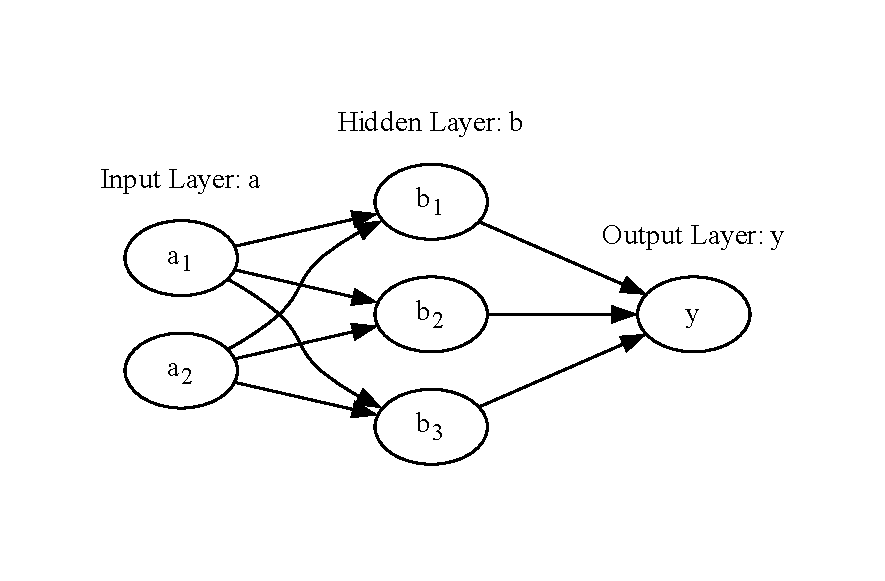
\includegraphics[width=0.5\textwidth]{graph/mlp}
  \label{fig:mlp} 
\end{figure}

Each node in b in the \ac{MLP} as seen in \figureref{fig:mlp} is calculated like the node y in \figureref{fig:perceptron}. That also means that every node combination between the layers has a weight. Such a combination of layers is called a fully connected layer. When there is a lot of correlation between all the nodes, then such a fully connected layer is useful as it is also fully utilized. However particularly when the nodes of the input layer represent the pixels of an image and the task is some form of recognition of objects in the image, most connections are not well utilized, since pixels that are further away from each other tend to have no meaningful connection \cite{aghdam2017guide}.

Convolutional layers work like a kernel based image filter but make the kernel trainable instead of static. This has the advantage that each convolutional neuron only processes data from its receptive field instead of the whole image. The receptive field of a neuron refers to the area of pixels in the source image that the data the neuron gets is dependent on. Using just one convolutional layer means that the neurons in the resulting tensor are just dependent on an area in the source image as big as the kernel of that convolution. Therefore \acp{CNN} tend to have many layers to be able to recognize larger shapes in the image. The resulting data of a convolutional layer is also called a feature map. 

\section{Shapely} % TODO: Add cites or footnotes in these sections

Shapely is a popular Python package for computational geometry. It provides a wide range of geometric objects and operations for working with planar geometric shapes, such as points, lines and polygons. Shapely is widely used in various domains, including geographic information systems, spatial data analysis, and computer graphics.

\section{Open CV}

\ac{OpenCV} is an open-source computer vision and machine learning software library designed for various computer vision tasks such as image processing and object detection. It was originally developed by Intel and later maintained by Willow Garage and Itseez. \ac{OpenCV} is written in C++ and has interfaces for C++, Python, and other programming languages.

\subsection{ArUco Detection}
\label{sec:aruco_det}

The \ac{ArUco} library implemented into \ac{OpenCV} is based on a paper from S. Garrido-Jurado et al. \cite{garrido2014automatic}. The \ac{ArUco} detection starts by using local adaptive thresholding on the image. Afterwards the Suzuki
and Abe algorithm \cite{SUZUKI198532} is applied to the thresholded image to extract the contours. The contours are then transformed into polygons \cite{douglas1973algorithms} and all polygons with more or less than 4 vertices are discarded. Then homographies for all remaining polygons are calculated such that the perspective on the potential marker is removed. The flattened image is then binarized using Otsu's method \cite{4310076}, which results in the lowest possible intra-class variance of black and white parts of the potential marker. Finally the marker is divided into a grid and further processed as a binary number based on the brightness of the grid cells.

This algorithm is however based on the assumption that the marker contour is always visible. If it is not, detections can become skewed or nothing is detected as seen in \figureref{fig:aruco-det}.

\begin{figure}
  \centering
  \subcaptionbox{An easily detectable \ac{ArUco} marker image}
     {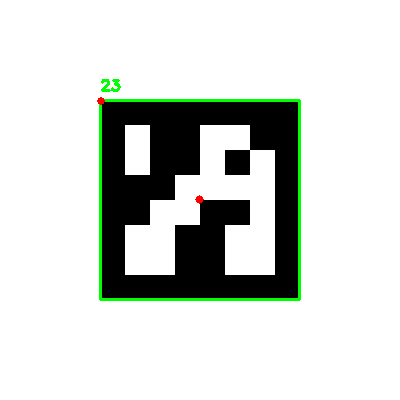
\includegraphics[width=0.3\textwidth]{image/rec}}
  \subcaptionbox{An \ac{ArUco} marker image with obscured contour corner}
     {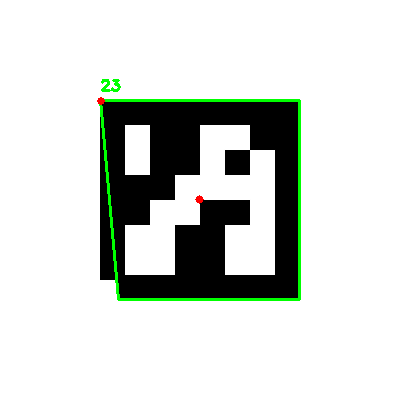
\includegraphics[width=0.3\textwidth]{image/skewed-rec}}
  \subcaptionbox{An \ac{ArUco} marker image with broken contour}
     {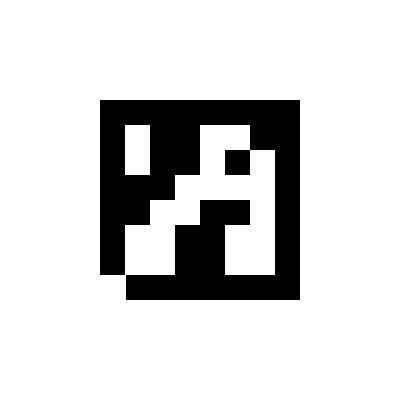
\includegraphics[width=0.3\textwidth]{image/no-rec}}
  \caption{Open CV ArUco Detection on example \ac{ArUco} images which have been partly obscured by a white rectangle}
  \label{fig:aruco-det}
\end{figure}

\section{Albumentations}

Albumentations is a Python library for image augmentation \cite{info11020125}. Image augmentation is a technique used to artificially expand a dataset by applying various transformations to the existing images. This helps improve the performance and generalization of machine learning models, especially in scenarios where the training data is limited. 

Albumentations was primarily build for high performance, such that its usage in dataloaders does not slow down the training process \cite{info11020125}. It transforms the image, as well as keypoint, bounding box and mask labels of the training sample, if the selected augmentation transformations support the label format. 

\section{Pytorch}

PyTorch is an open-source machine learning library for Python that has gained significant popularity in the deep learning and artificial intelligence research communities. Originally developed by Facebook's AI Research lab (FAIR) and now maintained by the Linux Foundation, PyTorch offers a flexible and dynamic computational graph, making it particularly well-suited for developing and training neural networks.

\section{SAHI}

The Python package \ac{SAHI} is a lightweight vision library designed to perform large scale object detection and instance segmentation \cite{akyon2022sahi,obss2021sahi}. It was developed to address the challenges of detecting small objects and performing inference on large images, which are common issues in practical usage. 

Fundamentally \ac{SAHI} uses a sliding window over the input image to split it into slices and lets the model predict objects in each of the slices of the image individually. Then it combines the predictions done on image slices into a prediction over the whole image. Since the slices may overlap there is support for bounding box prediction combination. Since models only see input images at a fixed resolution and smaller objects may disappear if the image is rescaled, this sliding window approach helps with detection on large images. 

\ac{SAHI} is framework agnostic and so can be modified to work with any model. However it has YOLOX, YOLOv5, YOLOv8, MMDetection and Detectron2 support by default.

\section{HyperOpt}

Hyperopt is a Python package designed for hyperparameter optimization, a fundamental aspect of machine learning model development \cite{bergstra2013making}. It systematically explores the hyperparameter space using a variety of optimization algorithms, most notably \ac{TPE}, aiming to discover the parameter combination that optimizes a predefined objective function. 

Hyperopt sees the objective function as a black box and makes few assumptions, which comes with flexibility but slower optimization than with loss functions in neural network training. Since the entire machine learning process is not a derivable function, this is the best choice for optimizing hyperparameters.

A combination of grid search and manual search are widely used to optimize hyperparameters. However it was shown that such processes tend to not be as efficient as sampling randomly from the hyperparameter space \cite{bergstra2012random}. \ac{TPE} is based on this realization as it behaves like random sampling in the first runs, but afterwards it uses the sampling history to find promising new parameter combinations \cite{bergstra2011algorithms}. 
% \ac{TPE} roughly works in these steps:

% \begin{enumerate}
%   \item Initialize the search space with Gaussian distributions or categorical distributions for continuous parameters and discrete parameters respectively.
%   \item Sample the objective function
%   \item The outputs of the objective function are thresholded into good and bad configurations
%   \item A exploitation \ac{PDF} is constructed for good configurations and a exploration \ac{PDF} is constructed for bad configurations
%   \item 
% \end{enumerate}

% TODO?: \section{Bounding Box conventions}

\section{mAP Scores}

\ac{mAP} scores are a class of commonly used metrics in the field of object detection to evaluate the performance of an object detection model \cite{padilla2020survey}. They aim to provide a measure of how well the model can identify and locate objects within an image. However there is a lack of consensus about the \ac{mAP} calculation. I will therefore focus on three popular \ac{mAP} scores. 

\subsection{IoU}

\begin{figure}
  \caption{Visualization of \ac{IoU} calculation}
  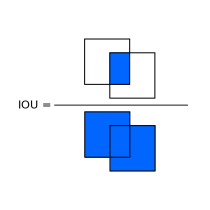
\includegraphics[width=0.5\textwidth]{image/iou}
  \label{fig:iou}
\end{figure}

The metric commonly chosen to measure the prediction quality between a prediction and ground truth label is the \ac{IoU} \cite{padilla2020survey}. The \ac{IoU} is a measurement based on the  Jaccard Index, a coefficient representing the similarity of two sets of data \cite{jaccard1901etude}. In the object detection context the \ac{IoU} measures the area of overlap divided by the area of union between two bounding boxes as shown in \figureref{fig:iou}.

\subsection{Precision and Recall}

In the context of object detection there exist three prediction cases, with the \ac{TN} case being omitted, since it applies to all possible bounding boxes that were not predicted, which depends more on the image resolution than the predictions, assuming the bounding box coordinates are integer values.

\begin{itemize}
  \item[$\bullet$] \ac{TP}: The highest confidence prediction of a ground truth label with an \ac{IoU} higher than the threshold
  \item[$\bullet$] \ac{FP}: An incorrect or imprecise prediction
  \item[$\bullet$] \ac{FN}: An undetected ground truth bounding box
\end{itemize}

Since \ac{TN} is not available in this context, metrics that use the \ac{TN} are also not available \cite{padilla2020survey}. Instead precision $P$ and recall $R$ are used as metrics.

$$P = \frac{TP}{TP + FP} = \frac{TP}{\text{all predictions}}$$

$$R = \frac{TP}{TP + FN} = \frac{TP}{\text{all ground truths}}$$

Precision measures the percentage of correct predictions among all predictions and recall measures the percentage of correct predictions among all ground truth boxes. 

The difference becomes most apparent when thinking about the extreme cases. If a model would output every possible bounding box on an image the recall would be 100\%, since for each ground truth bounding box there is an exact same prediction bounding box. If a model would instead output a perfect prediction for one ground truth bounding box and nothing for any other ground truth bounding boxes, the precision would be 100\%, since each made prediction is correct. Since both cases are undesirable but still result in an high score in one of the metrics a combination of both is needed.

\subsection{Table}

\begin{figure}
  \caption{Visualization of example prediction and ground truth bounding boxes}
  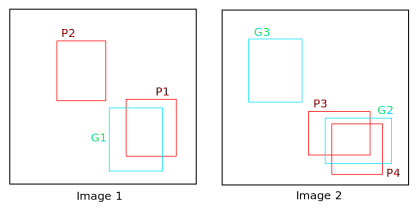
\includegraphics[width=0.8\textwidth]{image/preds}
  \label{fig:preds}
\end{figure}

The first part of the \ac{mAP} calculation are the same across all scores considered. That unified part of the computation is described here using the example\footnote{\url{https://kharshit.github.io/blog/2019/09/20/evaluation-metrics-for-object-detection-and-segmentation}, accessed on 08.10.2023} shown in \figureref{fig:preds}. 

Firstly a table of all predictions over all images in a given dataseries is created as seen in Table \ref{tab:mAP}. The table is sorted by prediction confidence. If there are multiple predictions for a single ground truth label, the prediction with the highest confidence is considered TP, if its \ac{IoU} is over the threshold, and all others FP, as seen with prediction P3. 

\begin{table}
  \begin{tabular}{ c c c c c c c c }
   Ground truth & Prediction & Confidence & TP & Acc. TP & Acc. FP & Precision & Recall \\ 
   \hline
   G2 & P4 & 98\% & Yes & 1 & 0 & 1 & 0.33 \\
   G2 & P3 & 89\% & No & 1 & 1 & 0.5 & 0.33 \\
   G1 & P1 & 78\% & Yes & 2 & 1 & 0.67 & 0.67 \\
   - & P2 & 60\% & No & 2 & 2 & 0.5 & 0.67 \\
   \hline
  \end{tabular}
  \caption{\label{tab:mAP}\ac{mAP} table of the example given in \figureref{fig:preds}.}
\end{table}

As the table is stepped through from highest confidence predictions to lowest, the accumulated TP and FP are incremented based on whether the prediction was correct or incorrect and saved into each table row \cite{padilla2020survey}. By computing $\text{acc \ac{TP}} / (\text{acc \ac{TP}} + \text{acc \ac{FP}})$ a preliminary precision is computed for each row. Similarly a preliminary recall value is calculated for each table row by dividing the accumulated \ac{TP} by the total number of ground truth labels of all images. Its important to note that recall values due to their computation formula here are monotonically increasing as the table rows are visited. When plotting the precision and recall values of the table rows as y and x components of points, the \ac{PR curve} is obtained as seen in \figureref{fig:pr-curve}.

\begin{figure}
  \caption{Example of a \ac{PR curve} plot taken from training with real data}
  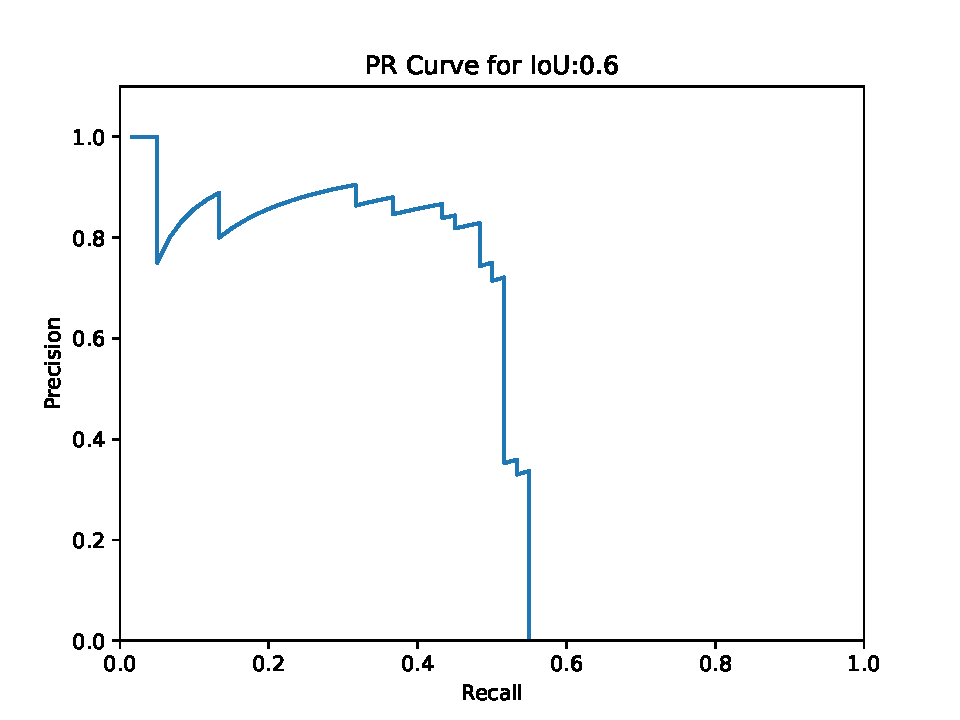
\includegraphics[width=0.8\textwidth]{image/eval_PR_Curve_0.60}
  \label{fig:pr-curve}
\end{figure}

The \ac{mAP} scores are now based on the \ac{AUC} of the \ac{PR curve}, which represents the desired combination of the precision and recall scores.

\subsection{Pascal VOC 2007}

For the VOC 2007 score the table as described earlier is computed for an \ac{IoU} threshold of 0.5 \cite{everingham2010pascal}. This threshold is deliberately set low to account for inaccuracies on the ground truth data, that can arise from hard to label objects. The VOC 2007 score summarizes the shape of the \ac{PR curve} by taking 11 equally spaced recall values . For each chosen recall value the maximum precision value on the curve at or to the right of that recall value is computed. Finally the AP score is defined as the mean of those maximum precision values as given by:

$$AP_{11} = \frac{1}{11} \sum_{r\in(0,0.1,...,1)}p_{interp}(r)$$

where

$$p_{interp}(r) = max_{\bar{r} : \bar{r} \geq r}p(r)$$

%$$p(r) = \text{the precision value on the \ac{PR curve} given a recall value}$$

Since I focus on the one class case for object detection eg. only on ArUco markers, that AP score is also the \ac{mAP} score here, otherwise the \ac{mAP} score would be the mean of the AP scores of all classes.

\subsection{Pascal VOC 2010}

The VOC 2010 score computes the \ac{PR curve} for an \ac{IoU} threshold of 0.5. It considers the \ac{PR curve} \ac{AUC} not just at 11 points but on all points of the table, giving this approach the name all-point interpolation \cite{padilla2020survey}. It is computed using the following formula:

$$AP_{all} = \sum_{n}(r_{n+1} - r_n)p_{interp}(r_{n+1})$$

where

$$p_{interp}(r_{n + 1}) = max_{\bar{r} : \bar{r} \geq r_{n+1}}p(\bar{r})$$

Since the VOC 2010 score takes all given recall values into account it is generally more accurate than the VOC 2007 score.

\subsection{Microsoft COCO}

The object detection part of the \ac{COCO} detection challenge defines multiple AP score types, such as AP across scales where the ground truth masks are split by their pixel area \cite{padilla2020survey}. However for this work I focused on the most used AP score definition of \ac{COCO}, which is the AP@50:5:95 score. It refers to the computation of multiple \acp{PR curve} using different \ac{IoU} thresholds. In this case 10 \ac{IoU} thresholds from 0.50 to 0.95 with a step width of 0.05 \cite{terven2023comprehensive}. \ac{COCO} also uses recall points, similar to the VOC 2007 score. However with 101 values instead of 11 between 0 and 1 with a step width of 0.01. %given by the following number series: ${0, 0.01, ..., 1}$. 
The \ac{COCO} mAP score, or average mean average precision score as proposed by Redmon et al., then refers to the average of the computed mAP scores for each \ac{IoU} threshold \cite{redmon2018yolov3}. 

The \ac{COCO} scores usefulness lies in its measurement of how tight a prediction bounding box is around a ground truth bounding box using higher \ac{IoU} thresholds. Both VOC scores described see a prediction as correct as soon as its \ac{IoU} is above 0.5 and make no difference between predictions with an \ac{IoU} of 0.55 or 0.9. The \ac{COCO} score therefore gives the opportunity to measure further improvements to trained models, assuming the ground truth labels of the dataset are accurate enough.

\chapter{Related Work}
\label{chap:relatedw}

In the following paragraphs papers focusing on difficult \ac{ArUco} marker detection using neural networks as well as papers focusing on image augmentation techniques are shortly introduced.

\section{ArUco Marker Detection}

\ac{ArUco} markers can usually be detected well enough for most usecases by \ac{OpenCV}'s own detection algorithm. However there are a number of more difficult usecases. In the following they are shortly introduced.

\subsection{UAV pose estimation}

Another use case in which robust detection of \ac{ArUco} markers is essential is for the control of \acp{UAV} during landing \cite{li2020aruco}. Here camera pose estimation can help locate the \ac{UAV} if \ac{ArUco} markers are layed out on the landing field. However during real world usage markers can become occluded and other visual artifacts can make detection difficult. Therefore Li et al used fine tuned versions of \ac{YOLO}v3-spp and \ac{YOLO}v3-tiny as marker detectors, since these \ac{CNN} based networks can be more stable than classic detection systems. For training the \ac{UAV} took off, floated and landed repeatedly and images were taken. The original 4000x2250 pixel images were resized to 1000x562 pixel for subsequent processing speed. To make the training data more realistic black and white objects were placed on the floor to simulate occluding objects. For the test set images were taken similarly but markers were partly occluded by laying a white paper cutout on top of it, with occlusion ratios from 10\% to 40\%. 

Markers in test images which had occluded borders still had high detection rates even at high cover ratios while markers in which the middle was occluded had worse detection rates, showing that the marker pattern itself was most important for \ac{CNN} detection \cite{li2020aruco}.

\subsection{Deep ChArUco}

Other papers, which focus on neural network aided detection of \ac{ArUco} markers, do not address occlusion. However Hu et al's paper on ChArUcoNet and RefineNet covers keypoint detection of the marker corners in an postprocessing step after the bounding box detection under low light conditions \cite{hu2019deep}. Therefore the augmentations also focus on noise, blur and brightness as well as shadow effects and a homographic transform. Deep ChArUco is able to detect the markers reliably even at higher darkness degrees while the \ac{ArUco} detection algorithm fails earlier. 

\subsection{Helping people with visual impairment}

A paper from Elgendy et al proposes a navigation system for people with visual impairment using \ac{ArUco} markers that are placed indoors \cite{elgendy2021novel}. A series of modified networks all based on \ac{YOLO}v3-tiny were trained on 600 photos, which were expanded and augmented on disk to 7200 images. The augmentations used here include 90 degree rotation, blur and lighting effects. The evaluations showed high detection accuracies with higher accuracies on the custom \ac{YOLO}v3 networks. The networks were also successfully deployed on a HTC desire 826.

\section{Training Image Augmentation}

Image Augmentation is of large importance for generalization. Since a model is build in training by optimizing the similarity of its output on training images to target output, it will also only perform well on examples it was trained on or that are similar. Through variation in training, models can attain a level of generalization that allows them to perform well despite differences in lighting, occlusion, background, scale, etc. \cite{shorten2019survey}. A lack of such an ability of generalization leads to previously working models being unable to classify images if a single pixel changes color \cite{8601309}. Often this variation can come from a large dataset, but if real data is in short supply or if the labeling is too time consuming, image augmentation can replace it.

Image augmentations can be any kind of image transformation. However depending on the task and the dataset the effectiveness of different types of augmentations can vary dramatically. Nonetheless in the following I will introduce available papers with empirical comparisons or meta analyses of image augmentations.

\subsection{Comparison of augmentations on the Caltech101 dataset}

On the Caltech101 dataset using a custom classification \ac{CNN} Taylor et al. found that cropping improves the accuracy scores significantly while most other types of augmentation including custom augmentation types improve the score slightly as seen in Table \ref{tab:taylor-acc} \cite{8628742}.

\begin{table}
  \begin{tabular}{ c c c }
    & Top-1 Accuracy & Top-5 Accuracy \\ 
   \hline
   Baseline & $48.13 \pm 0.42\%$ & $64.50 \pm 0.65\%$ \\
   Flipping & $49.73 \pm 1.13\%$ & $67.36 \pm 1.38\%$ \\
   Rotation & $50.80 \pm 0.63\%$ & $69.41 \pm 0.48\%$ \\
   Cropping & $61.95 \pm 1.01\%$ & $79.10 \pm 0.80\%$ \\
   Color Jittering & $49.57 \pm 0.53\%$ & $67.18 \pm 0.42\%$ \\
   Edge Enhancement & $49.29 \pm 1.16\%$ & $66.49 \pm 0.84\%$ \\
   Fancy PCA & $49.41 \pm 0.84\%$ & $67.54 \pm 1.01\%$ \\
   \hline
  \end{tabular}
  \caption{\label{tab:taylor-acc}Results of augmentation comparison from Taylor et al. \cite{8628742}.}
\end{table}

\subsection{Comparison of augmentations for detection of COVID-19 Pneumonia}

For automated detection of COVID-19 pneumonia in Chest X-rays Elgendi et al. empirically tested different combinations of augmentations from other related papers on three datasets with 10-fold cross validation of Chest X-ray images \cite{elgendi2021effectiveness}. They used 17 different pertained neural networks for transfer learning on this binary classification task and used the average score of the resulting 17 models given a combination of augmentations as the score of that combination. The following augmentations were considered:

\begin{itemize}
  \item[$\bullet$] Reflection
  \item[$\bullet$] Scaling
  \item[$\bullet$] Shearing
  \item[$\bullet$] Translation
  \item[$\bullet$] Rotation
\end{itemize}

While not using any augmentations led to the best score for this task and on these datasets, an augmentation pipeline consisting of reflection, translation and rotation got the second best score. The worst score was attained by an augmentation pipeline consisting of shearing, translation and rotation. 

Elgendi et al. also asked radiologists whether the augmentations used here made sense in the context of pneumonia detection and the opinions of the augmentations matched the empirical results. Elgendi et al. were even able to improve the performance of models from on of their earlier papers also covering detection on chest X-rays by removing any image augmentation \cite{elgendi2020performance, elgendi2021effectiveness}.

They conclude that \cite[optimization over each geometric augmentation is needed. For example, defining an “acceptable” range of rotation.]{elgendi2021effectiveness}

\subsection{Comparison of augmentations on aerial image labeling}

As part of the paper that introduced Albumentations Buslaev et al. showed the usefulness of Albumentations augmentations on the Inria Aerial Image Labeling dataset \cite{info11020125,maggiori2017can}. They applied random crop to a random square patch size of $[384;640]$ and resized the cropped region to an image size of 512x512. Afterwards they used augmentations bundled into none, light, medium and heavy on the images.

\begin{enumerate}
  \item No augmentations: no further changes to the image
  \item Light augmentations: Random horizontal flips, change of brightness, change of contrast, change of color, random affine transformation, random perspective transformation
  \item Medium augmentations, extending Light with: Gaussian blur, sharpening, coarse dropout, removal of some buildings, randomly generated fog
  \item Hard augmentations, extending Medium with: Random rotation by 90 degrees, image grid shuffle, elastic transformations, gamma adjustments, and contrast-limited adaptive histogram equalization
\end{enumerate}

\begin{table}
  \begin{tabular}{ c c c c c c }
   Augmentations & Train IoU & Valid IoU & Best Epoch & Data Time (sec/batch) & Model Time (sec/batch) \\ 
   \hline
   None & 84.67 & 73.89 & 45/100 & 0.09 & 0.6\\
   Light & 84.84 & 77.50 & 90/100 & 0.09 & 0.6\\
   Medium & 83.52 & 76.94 & 96/100 & 0.11 & 0.6\\
   Heavy & 79.78 & 78.34 & 95/100 & 0.13 & 0.6\\
   \hline
  \end{tabular}
  \caption{\label{tab:alb-iou}Results of augmentation comparison from Buslaev et al. \cite{info11020125}.}
\end{table}

With more augmentations on this dataset the validation \ac{IoU} score improved and the training epoch with the best validation \ac{IoU} was later, indicating that overfitting was prevented, as seen in Table \ref{tab:alb-iou}.

\subsection{Survey of common image augmentations}

Khalifa et al. compiled image augmentation techniques used in other papers \cite{khalifa2022comprehensive}. In the medical domain, which this work is the most similar to, \ac{GAN} and rotation techniques appear the most with each of them being used in three papers of the nine considered. Reflection and shifting operations were both used in two papers each.

\chapter{Networks}
\label{chap:netw}

This chapter introduces network architectures that I used for the \ac{ArUco} marker detection and their history. Since the models are supposed to run on smart phones, they should be as small as possible. Furthermore inference in real time would make the usage easier. Since both of these constraints mirror the strengths of the \ac{YOLO} network architectures, a majority of this chapter will focus on them.

\section{First YOLO Versions}

\ac{YOLO} is a popular object detection model that was first introduced by Joseph Redmon et al. in 2016 \cite{redmon2016you}. Two-stage detection models, such as R-CNN, were the standard at the time. They first propose regions of interest and then classify these regions. \ac{YOLO} however is a single-shot detector that processes the entire image in a single pass, making it faster and more efficient. The network structure of \ac{YOLO} can be seen in \figureref{fig:yolo}.

\begin{figure}
  \caption{Visualization of the most important layers of the \ac{YOLO} network, with the tensor width and height being mapped by $x \mapsto x^{0.7}$ and tensor length, eg. the feature map length, being scaled by $x \mapsto x^{0.5}$, the purple box denotes two fully connected layers, inspired by the visualization from Redmon et al. \cite{redmon2016you}, created using a modified version of the \href{https://github.com/jnccd/PlotNeuralNet}{PlotNeuralNet tool} \cite{haris_iqbal_2018_2526396}}
  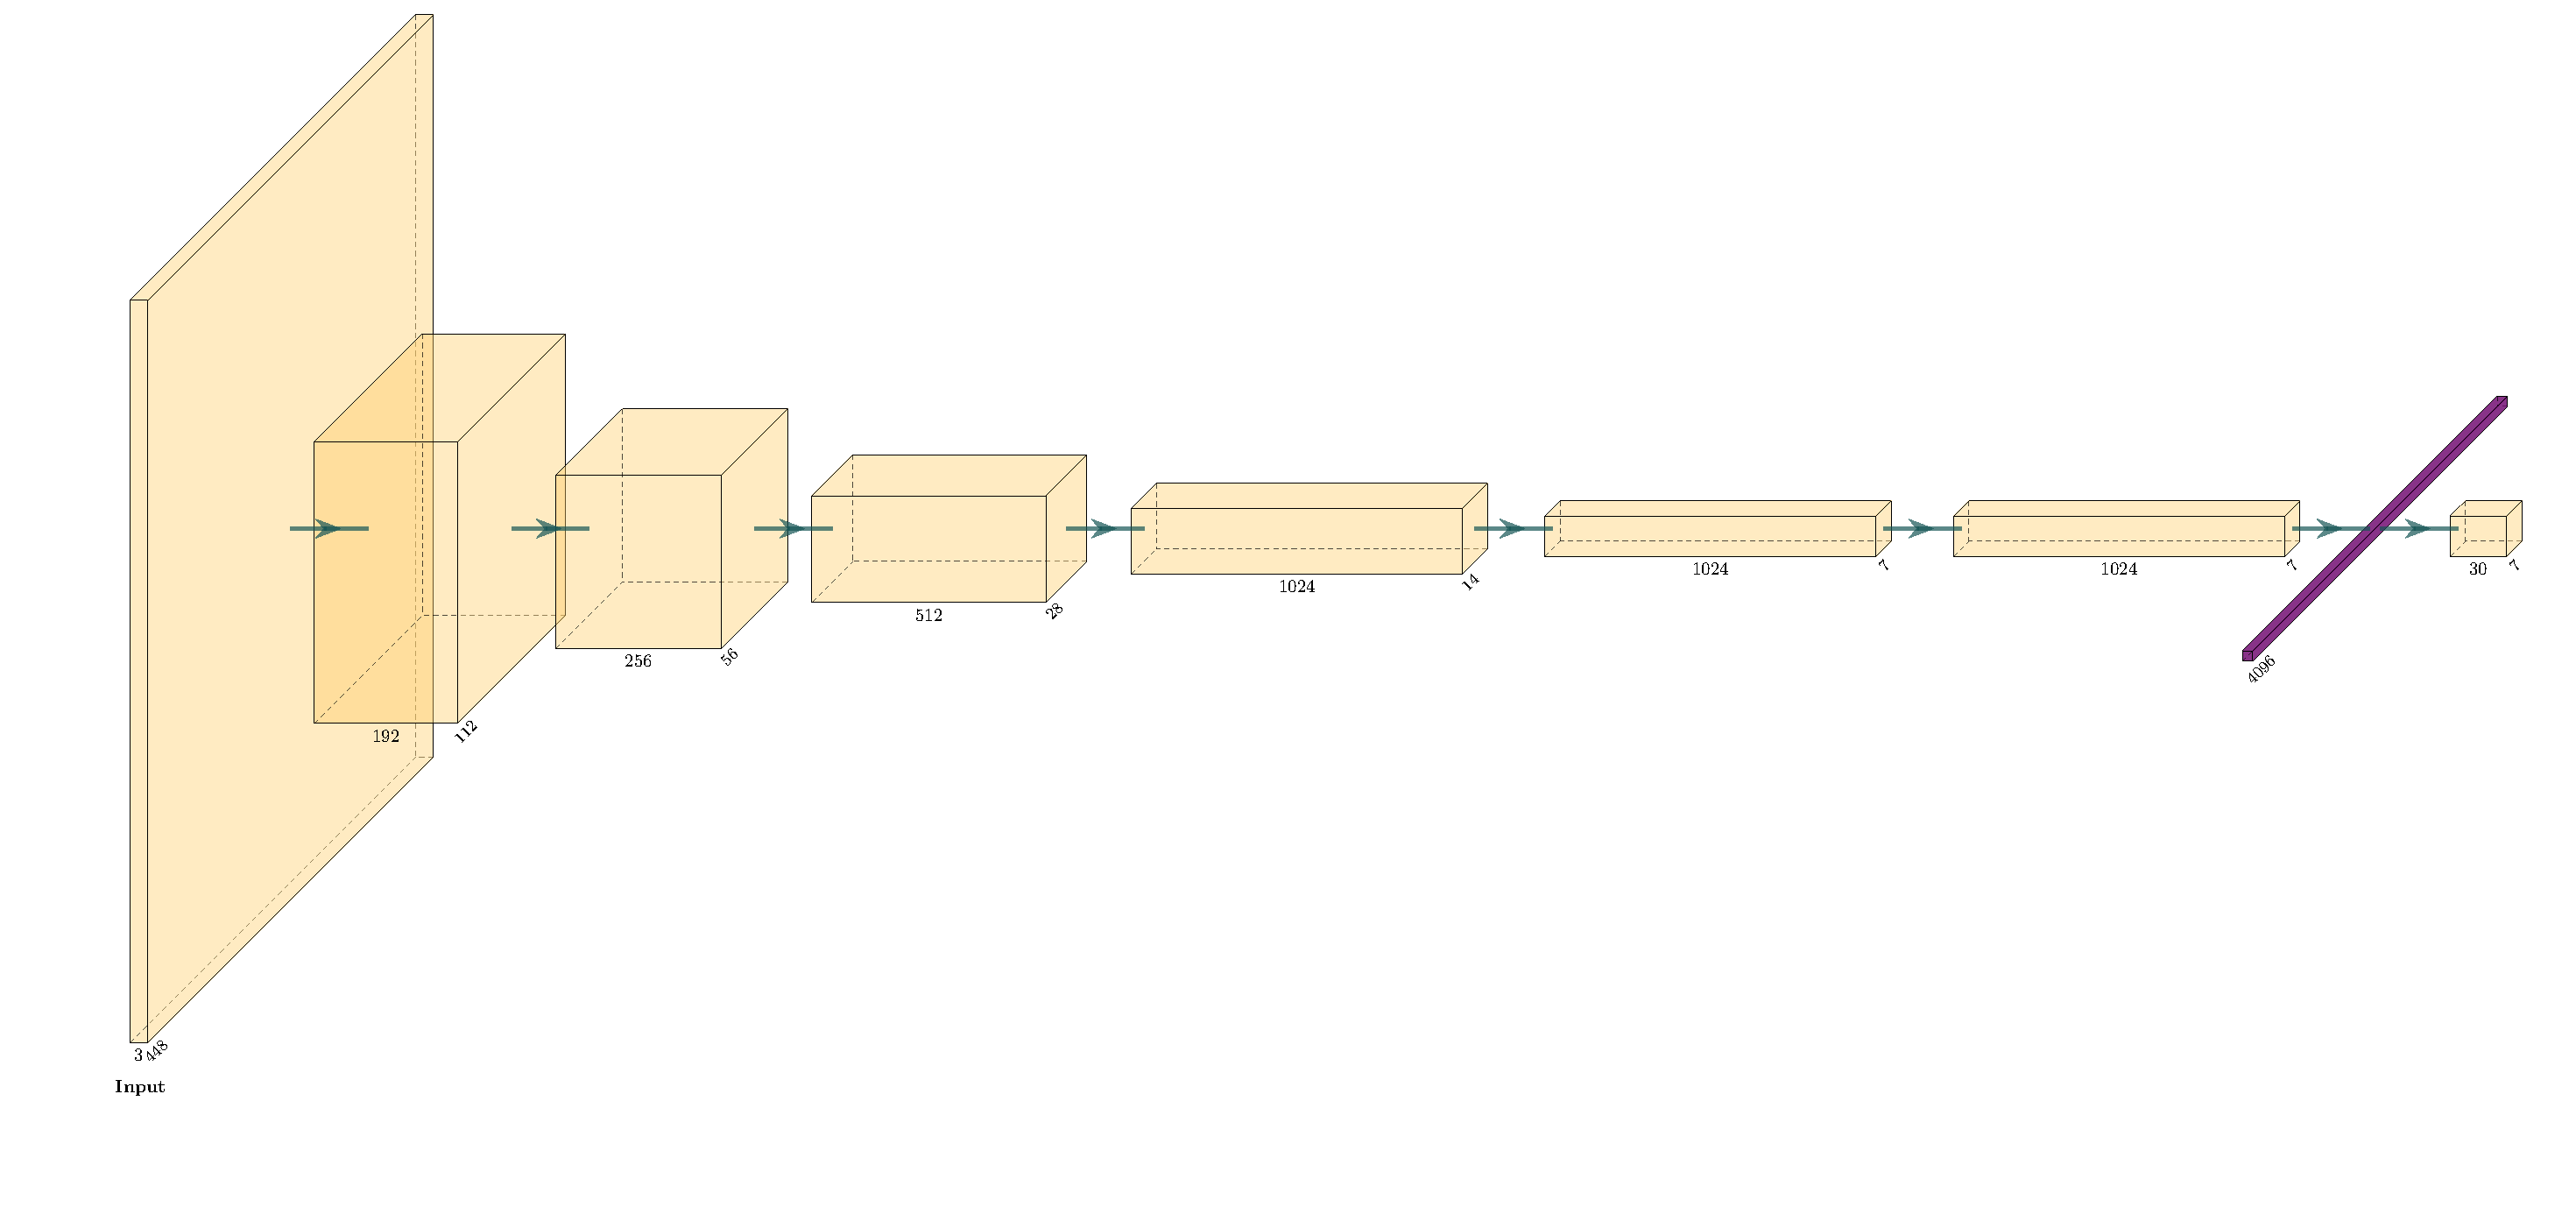
\includegraphics[width=\textwidth]{image/yolo}
  \label{fig:yolo}
\end{figure}

\ac{YOLO}v2 or \ac{YOLO}9000 improves on \ac{YOLO} with the introduction of anchor boxes, allowing the network to detect objects in regions of the image instead of the whole image at once \cite{redmon2017yolo9000}. Furthermore all fully connected layers are removed from the \ac{YOLO}v2 network architecture and the output of one of the earlier layers is passed through and concatenated into one of the last layers as seen in \figureref{fig:yolov2}. The first 23 layers (or 6 boxes in the figure) of the network are also referred to as the Darknet19 backbone, while the last 4 layers are the detection head. \ac{YOLO}v2 also introduced multi-scale training, meaning it can adapt its network size to different input image sizes from $320 \times 320$ to $608 \times 608$, as well as batch normalization and a better loss function.

\begin{figure}
  \caption{Visualization of the most important layers of the \ac{YOLO}v2 network, with the tensor width and height being mapped by $x \mapsto x^{0.7}$ and tensor length, eg. the feature map length, being scaled by $x \mapsto x^{0.5}$ created using a modified version of the \href{https://github.com/jnccd/PlotNeuralNet}{PlotNeuralNet tool} \cite{haris_iqbal_2018_2526396}}
  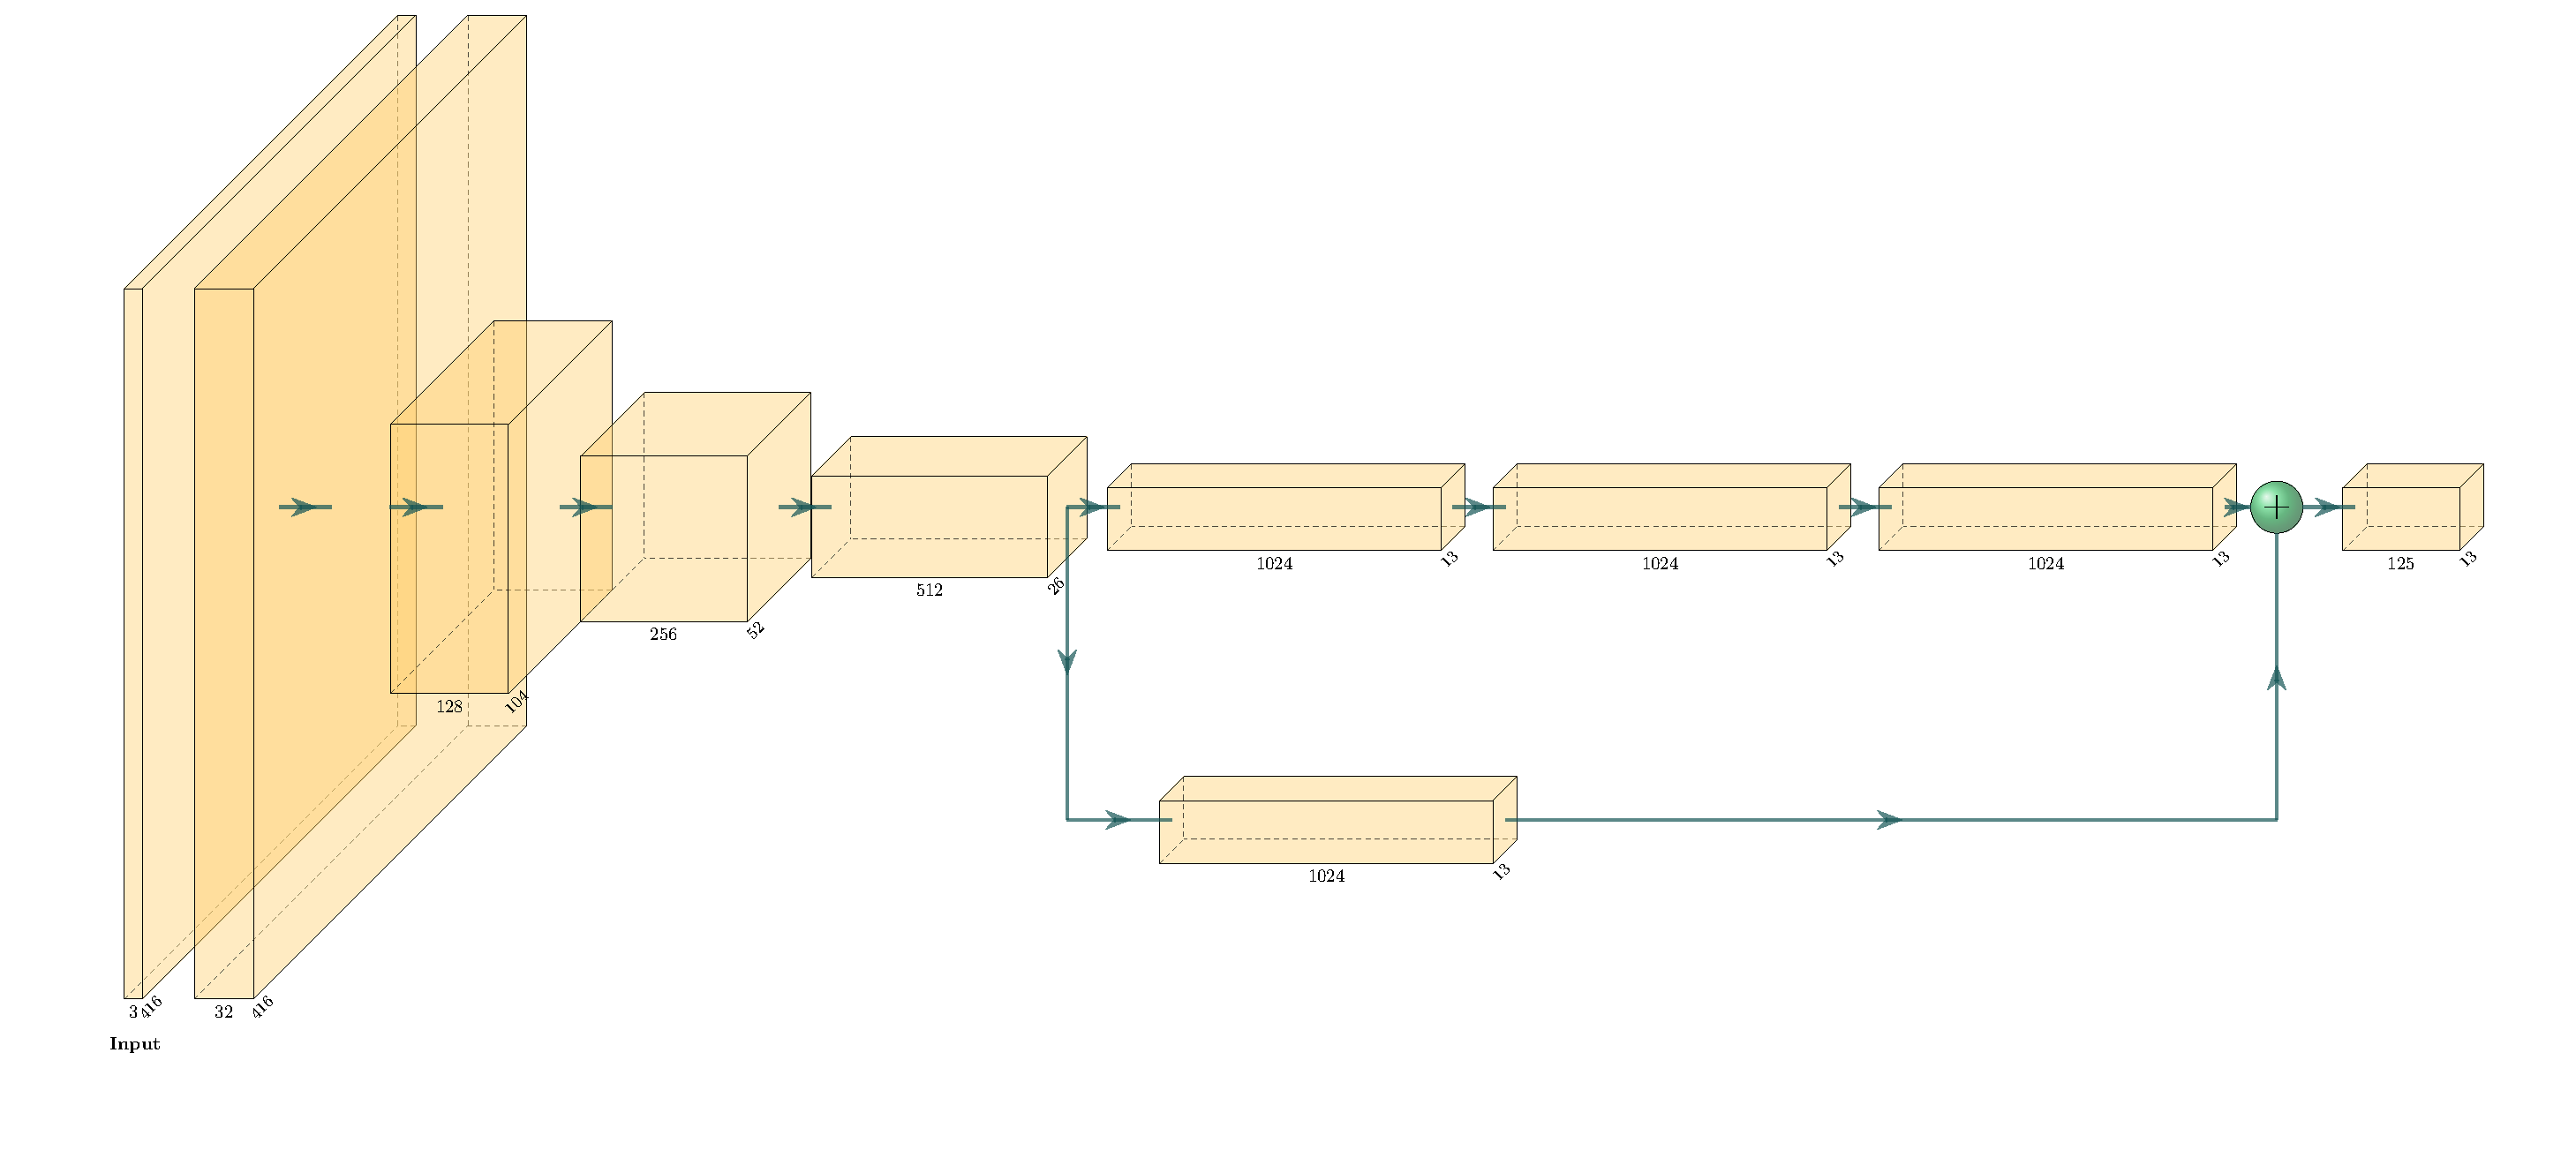
\includegraphics[width=\textwidth]{image/yolov2}
  \label{fig:yolov2}
\end{figure}

\ac{YOLO}v3 mainly improves the network architecture by developing approaches from \ac{YOLO}v2 and Darknet-19 further to create the Darknet-53 backbone, which got its name from the 53 convolutional layers it contains \cite{redmon2018yolov3}. \ac{YOLO}v3 also introduced a more efficient loss function and \ac{SPP}, which allowed it to detect bounding boxes at different scales more effectively \cite{jani2023model}.

\section{YOLO Versions Timeline}

\begin{figure}
  \caption{A timeline showing different \ac{YOLO} versions over time, based on the timeline from Terven et al. \cite{terven2023comprehensive}}
  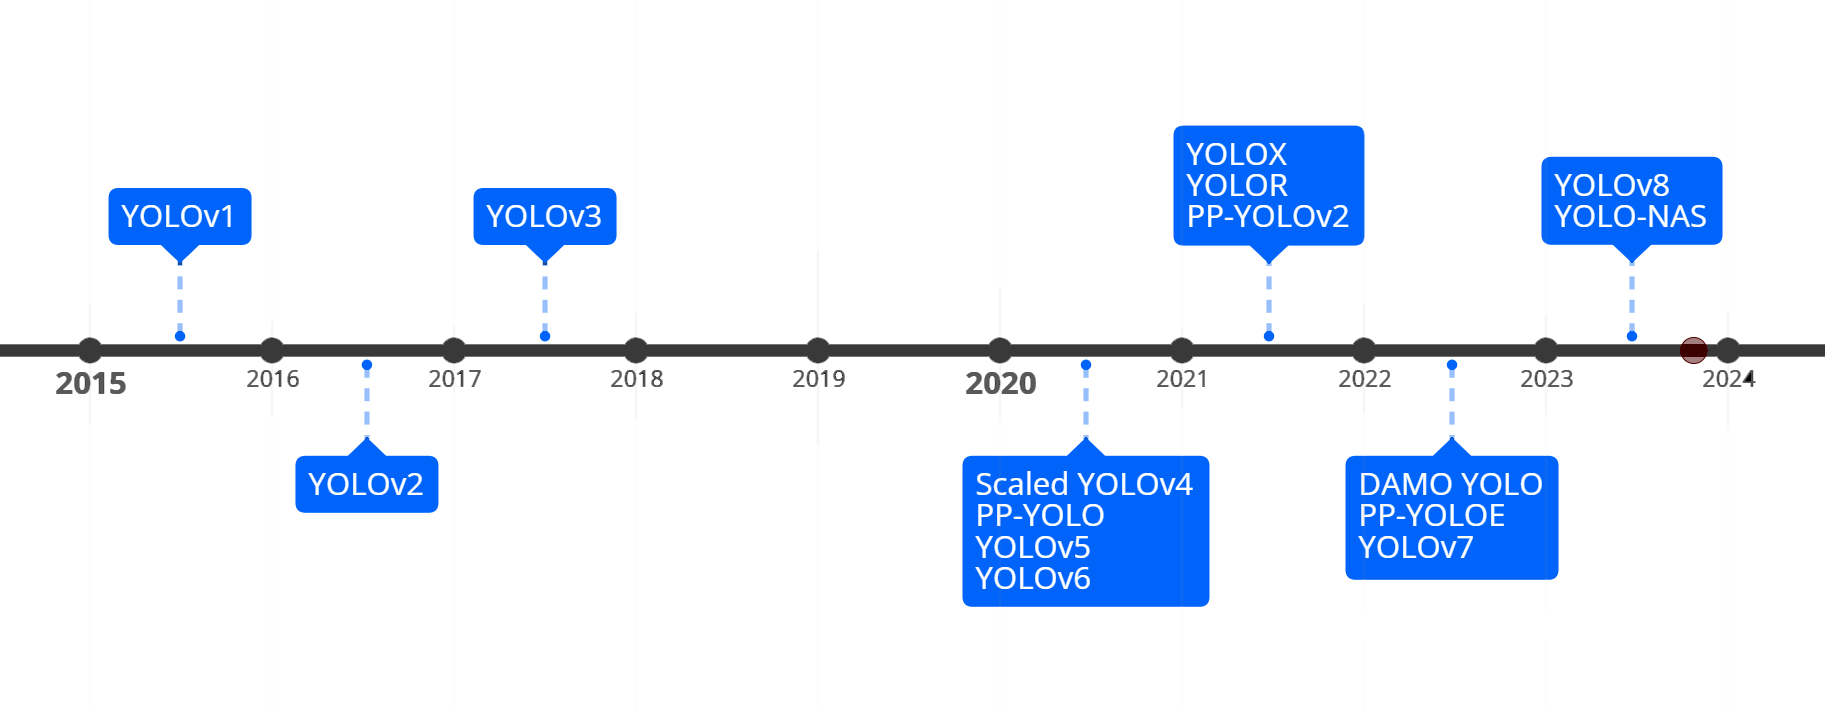
\includegraphics[width=\textwidth]{image/timeline_fix}
  \label{fig:yolo_timeline}
\end{figure}

While the first three \ac{YOLO} versions were developed by the same developers, starting with \ac{YOLO}v4 various developers started releasing \ac{YOLO} versions. A full timeline of the releases can be seen in \figureref{fig:yolo_timeline}. For this work I will focus on \ac{YOLO}v5, due to its popularity and its plentiful resources, as well as \ac{YOLO}v8 and \ac{YOLO}-NAS due to their recency and \ac{YOLO}v8's similarity to \ac{YOLO}v5.

\section{YOLOv5}

%instead of the developers of the first three \ac{YOLO} versions
\ac{YOLO}v5 was developed by Ultralytics and further increased the mAP detection score on the COCO dataset through small changes to the architecture, new box coordinates, a build target process as well as new augmentation techniques\footnote{\url{https://docs.ultralytics.com/yolov5/tutorials/architecture_description}, accessed on 20.10.2023} \cite{gjocher2022yolov5,terven2023comprehensive}. \ac{YOLO}v5 also made hyperparameter optimization easier and added quality of life features. \ac{YOLO}v5 provides models in five different sizes: \ac{YOLO}v5n (nano), \ac{YOLO}v5s (small), \ac{YOLO}v5m (medium), \ac{YOLO}v5l (large), and \ac{YOLO}v5x (extra large).

\subsection{Architecture}

\ac{YOLO}v5's network architecture consists of a backbone, a neck and a head which are connected to each other in that order \cite{jani2023model}. \ac{YOLO}v5's backbone is the CSP-Darknet53 structure, which was the structure that \ac{YOLO}v4 used \cite{bochkovskiy2020yolov4}. \ac{YOLO}v5's Neck consists of the SPPF, which is a more efficient version of \ac{YOLO}v3's \ac{SPP}, and new \ac{CSP-PAN} structures, which improve the information flow through the network \cite{liu2018path}. \ac{YOLO}v5 uses the same head structure as \ac{YOLO}v3 at the end of the network. The entirety of the network is visualized in \figureref{fig:yolov5}.

\begin{figure}
  \caption{Visualization of the most important layers and blocks of the entire \ac{YOLO}v5 network, with the tensor width and height being mapped by $x \mapsto x^{0.7}$ and tensor length, eg. the feature map length, being scaled by $x \mapsto x^{0.5}$, created using a modified version of the \href{https://github.com/jnccd/PlotNeuralNet}{PlotNeuralNet tool} \cite{haris_iqbal_2018_2526396}}
  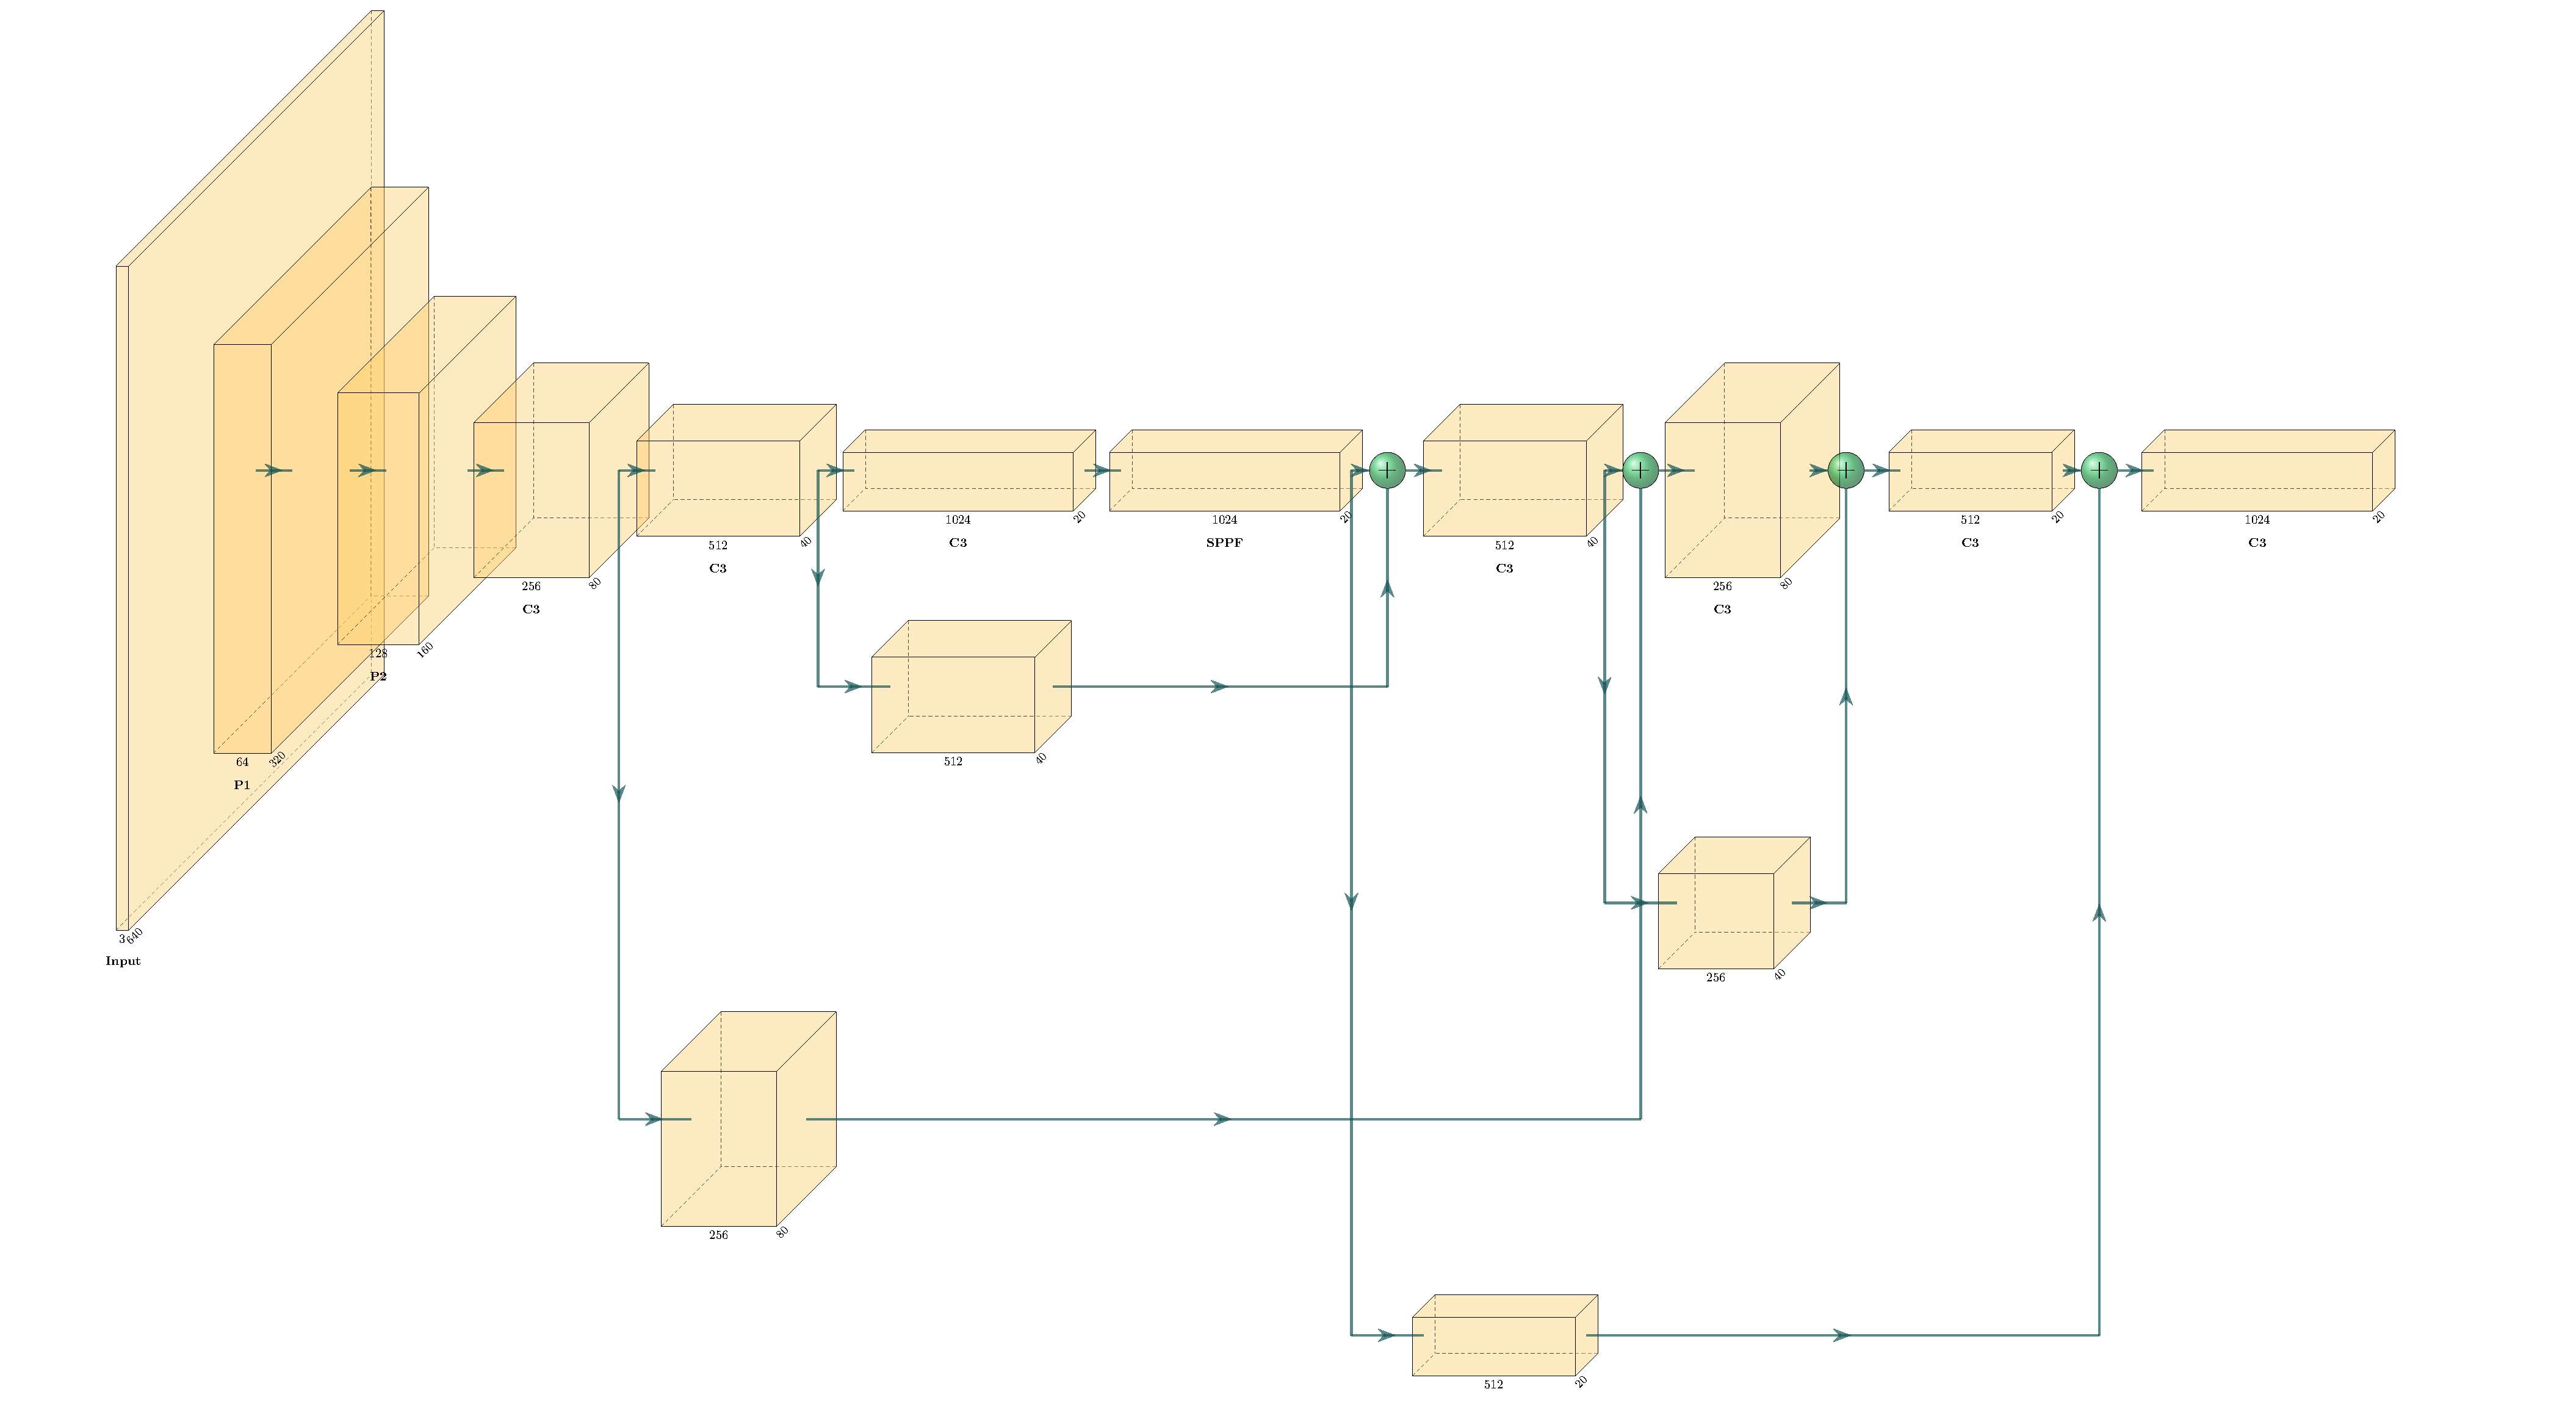
\includegraphics[width=\textwidth]{image/yolov5}
  \label{fig:yolov5}
\end{figure}

\subsection{Built-in Data Augmentation}

\ac{YOLO}v5 also comes with predefined augmentation techniques. 

\begin{itemize}
  \item Mosaic Augmentation: This technique places four training images next to each other in one bigger image.
  \item Random Affine Transformations: This technique applies random rotation, scaling, translation, and shearing to the image.
  \item HSV Augmentation: This technique applies random changes to the Hue, Saturation, and Value of pixels within a certain range for each of the values.
  \item Random Horizontal Flip: This technique randomly flips the image around the y axis.
\end{itemize}

\ac{YOLO}v5 further defines augmentations such as Copy-Paste Augmentation and MixUp Augmentation. However these augmentations were disabled by default and not used over the course of this thesis.

\section{YOLOv8}

\ac{YOLO}v8 is the second \ac{YOLO} version from Ultralytics and provides multiple models in the same sizes as \ac{YOLO}v5\footnote{\url{https://docs.ultralytics.com/models/yolov8/}, accessed on 24.10.2023} \cite{terven2023comprehensive}. \ac{YOLO}v8 is anchor-free, which simplifies the training and decoding process. For the bounding box loss \ac{YOLO}v8 uses \ac{CIoU} \cite{zheng2020distance}, which besides the overlap area is also based on the central point distance and aspect ratio of the bounding boxes, as well as \ac{DFL} \cite{li2020generalized}. \ac{YOLO}v8 also provides a segmentation model.

\section{YOLO-NAS}

\ac{YOLO}-NAS was developed by Deci, which develops production grade models \cite{terven2023comprehensive}. The architecture of \ac{YOLO}-NAS was found by Deci's proprietary \ac{NAS} technology AutoNAC and comes in three sizes: \ac{YOLO}-NAS-S, \ac{YOLO}-NAS-M and \ac{YOLO}-NAS-L. The \ac{YOLO}-NAS models were pre-trained on the Objects365 dataset, which is newer and larger than the COCO dataset and gets its name from its 365 object categories \cite{shao2019objects365}. Afterwards they were trained on the COCO dataset.

% TODO?: \section{MobileNetV2}

\section{ViTs}

After the application of transformer blocks in natural language processing was successful they were also introduced into other domains, such as visual processing, resulting In \acp{ViT}. The application of transformers on vision tasks works by slicing the input image into many patches \cite{dosovitskiy2020image}. The pixel data of these patches is  further divided and interpreted as word vectors. These "visual words" can then be fed into a transformer based network. 

\acp{ViT} mark the newest major change in network architecture for the object detection task. The advantage of \acp{ViT} is their scalability, making \cite[models of unprecedented size]{dosovitskiy2020image} trainable. However in this work I aim to develop a detection system that would preferably run directly on patients smart phones, making large models impractical. Furthermore development on ConvNeXt showed that, when trained using similar modern training techniques, large convolutional networks can perform similarly well or better than vision transformers, therefore the improvements may not stem from network architecture itself \cite{liu2022convnet}.

% TODO?: \section{Unet}

\chapter{Methodology and Implementation}
\label{chap:implement}

In this chapter I describe how I structured my code and why as well as the core ideas of some algorithms. Furthermore I describe the hardware that was used for training.

\section{Goals}

% TODO: Talk about the whole image and pet parts of the inference pipeline here

My goal for the implementation is to write a software framework that allows me to train the custom data given to me on a wide variety of \acp{NN} using a wide variety of training techniques and to evaluate the effectiveness of all these approaches.

\section{Development Environment}

Most training for this work was done on the 'lena' server of the \ac{MIP} working group of the Kiel University. This server contains 128GB RAM and eight Nvidia GeForce RTX 2080Ti \acp{GPU} with 12GB VRAM each. Local training was done on a computer with 32GB RAM and a Nvidia GeForce RTX 3060Ti \ac{GPU} with 8GB VRAM.

Training on the server was done using a Docker Image and locally it was done in a conda environment. During development I used both TensorFlow and PyTorch, so for simplicity I chose to install them both in the same environments. This is possible because both the PyTorch version 2.0.1 and the TensorFlow version 2.12 depend on the same \ac{CUDA} Toolkit version 11.8 as well as on the \ac{cuDNN} version 8.4.1.50.

\section{Classic Approaches}

To validate that a neural network based approach is necessary in this case, I tested some approaches using algorithms from \ac{OpenCV}, that do not require machine learning. For these tests I chose a test image from the given data, on which the markers were facing the camera and had as much visible contours as possible, which can be seen in \autoref{fig:classic_base_img}. 

\begin{figure}
  \caption{Test Image for Classic Approaches}
  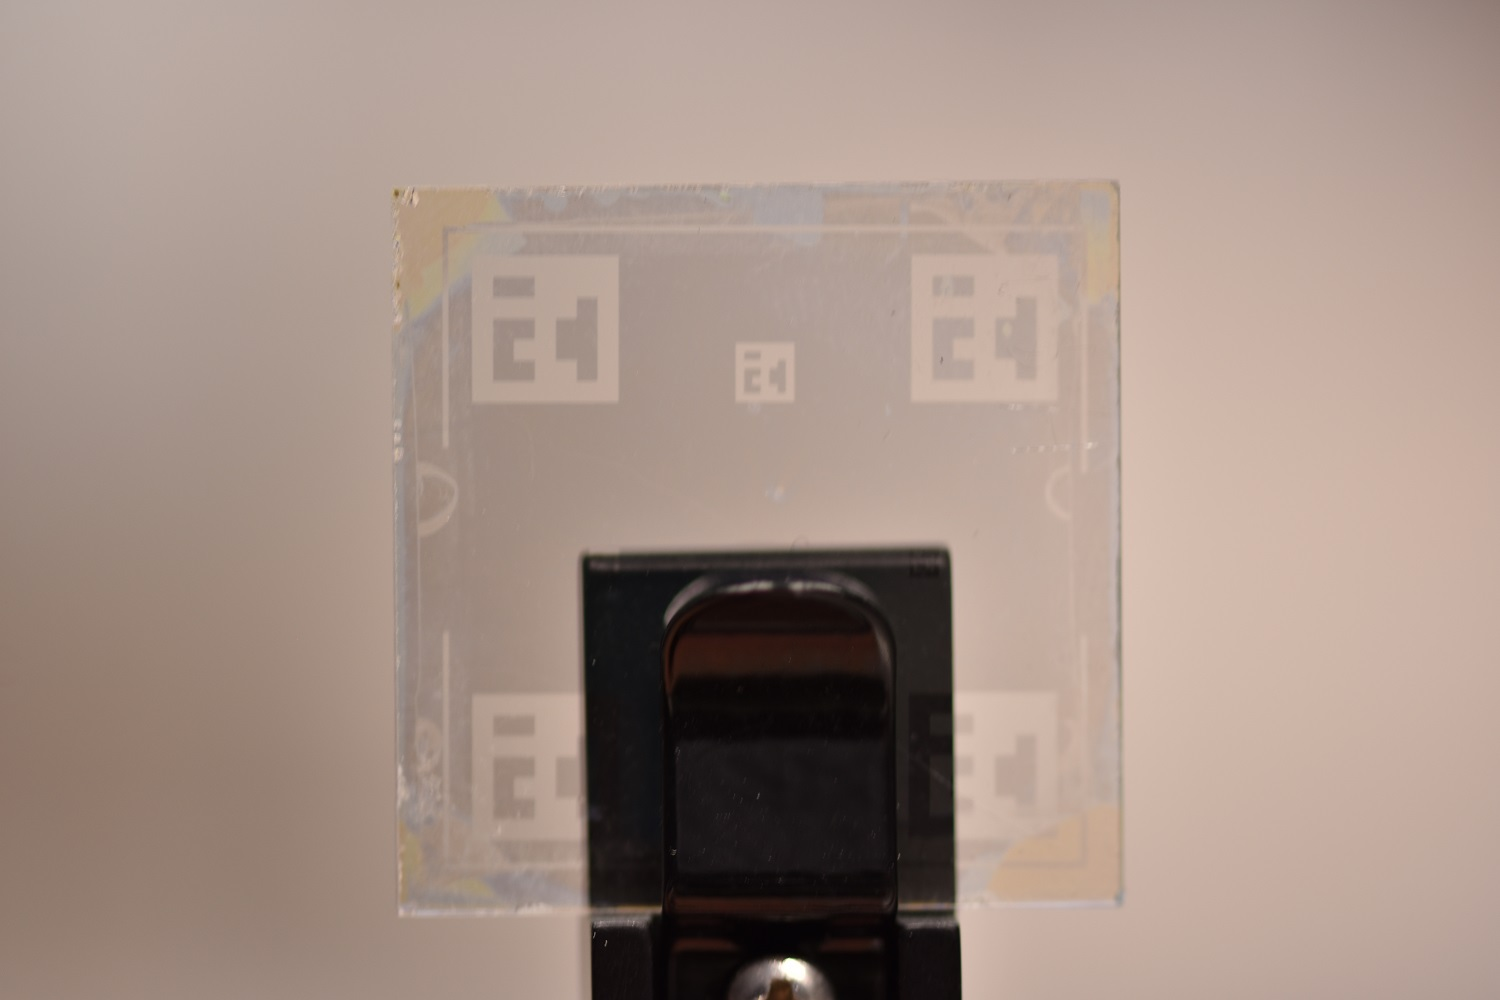
\includegraphics[width=0.7\textwidth]{image/classic_base_img}
  \label{fig:classic_base_img}
\end{figure}

\subsection{Open CV ArUco Detection}

\begin{figure}
  \centering
  \subcaptionbox{Detection Output with 4 Vertex Filter}
     {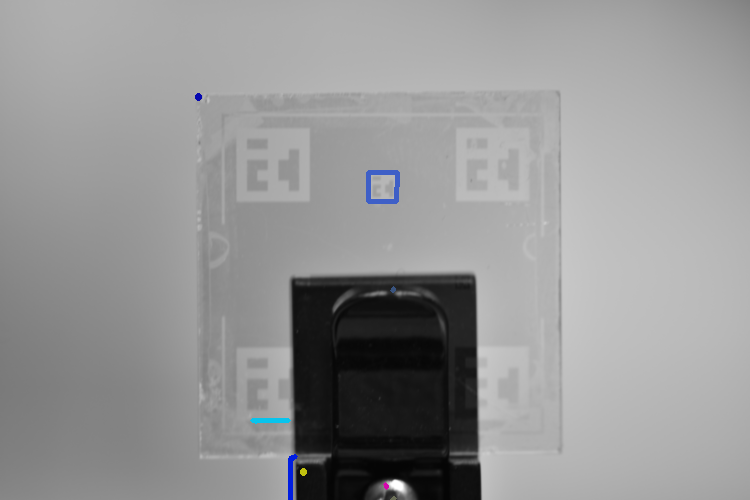
\includegraphics[width=0.4\textwidth]{image/classic_base_img_opencv_det_small}}
  \subcaptionbox{Detection Output without Filter}
     {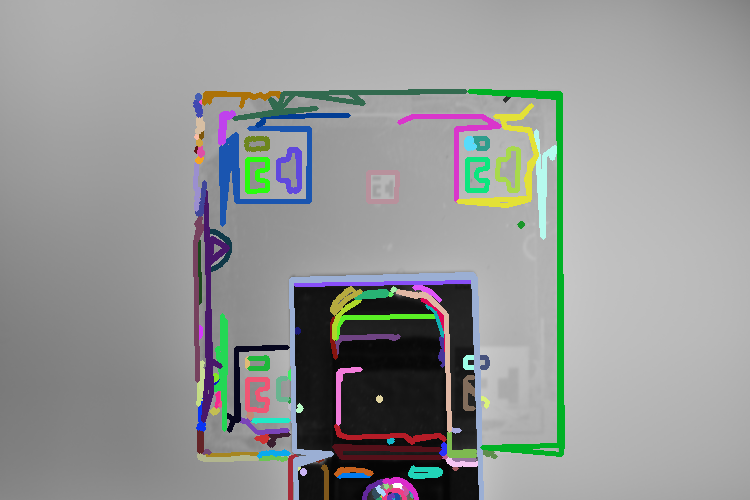
\includegraphics[width=0.4\textwidth]{image/classic_base_img_opencv_det_all}}
  \caption{Detections of the \ac{OpenCV} pipeline, with each polygon colored in a random color to make them distinguishable}
  \label{fig:classic_base_img_opencv}
\end{figure}

The built-in \ac{OpenCV} \ac{ArUco} detector does not detect any markers in the chosen base image. To find out why, I roughly recreated the \ac{ArUco} detector using \acp{OpenCV} built-in algorithm implementations up until the polygon creation step. The recreated pipeline mainly consists of the canny edge detector and the \texttt{findContours} and \texttt{approxPolyDP} methods applied to each level of an image pyramid. 

When filtering for only polygons with four vertices, the small polygon is detected on one scale, as seen on \autoref{fig:classic_base_img_opencv} (a). The better detection accuracy here may be due to cherry picked parameters. Without the filter in \autoref{fig:classic_base_img_opencv} (b), the problems of the polygon detection become apparent, as the contours of the markers in the image are not complete, which may in part explain the findings in \autoref{sec:aruco_det}.

\subsection{Histogram}

The idea of the histogram approach is, that the pixel gradient histogram distributions in a window around the marker in the image should have a similar distribution on each of the markers.

\begin{figure}
  \centering
  \subcaptionbox{Output of Histogram Difference, with the top left marker being the histogram baseline}
     {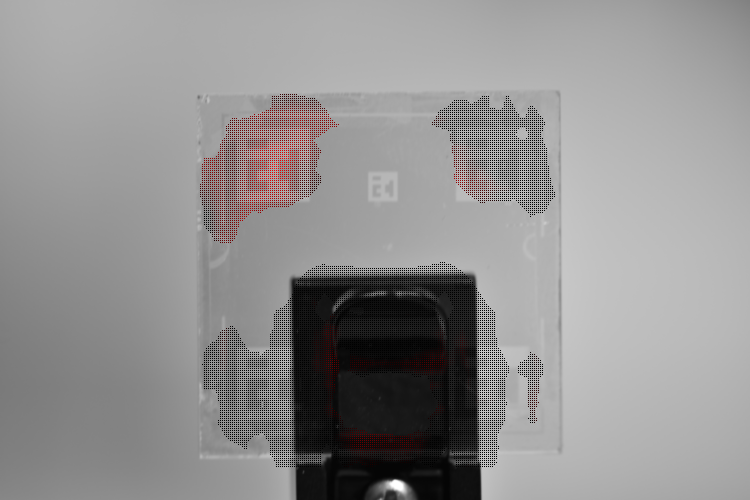
\includegraphics[width=0.4\textwidth]{image/classic_hist_markerynesses}}
  \subcaptionbox{Output of Histogram Peak based Score}
     {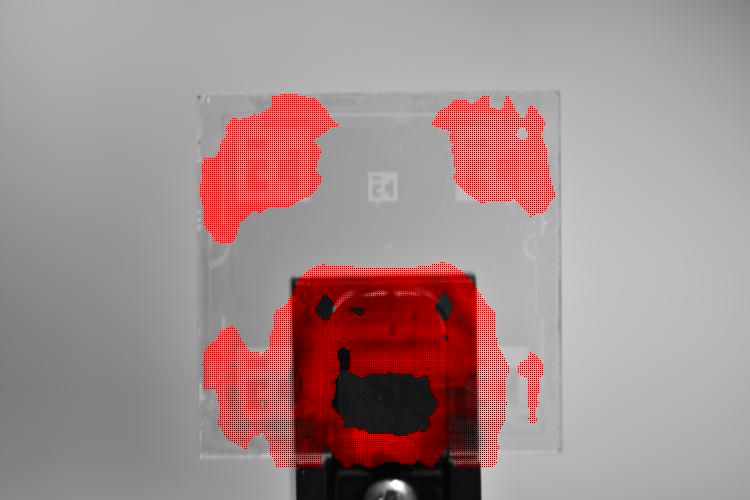
\includegraphics[width=0.4\textwidth]{image/classic_markeryness}}
  \caption{Output of the Histogram based Approach, where the pixels of middle points of all windows that passed the candidate check are repainted, the redness of the repainted pixel represents the score of its window}
  \label{fig:markeryness_scores}
\end{figure}

For this approach firstly the image is again scaled in different steps in an image pyramid. For each entry in the image pyramid, a thresholded version is computed using adaptive thresholding, as well as the image gradients in x and y direction and polar coordinate versions of the gradients. Afterwards the image is traversed with a 64x64 pixel window on a 2 pixel step width on the x and y axis. Then the script checks for each such window on the image if it is a candidate for the marker by checking the ratio of white to black pixels. If the window around a point in the image passes the candidate check, a histogram of size 20 is computed from the angles of the pixels in the window of the polar gradient array. Then the histogram difference between the known histogram on the middle of the marker on the top left and the current histogram is computed. The result of that computation can be seen in \autoref{fig:markeryness_scores} (a). 

There are many possible variations of this approach, such as also using the magnitude of the gradient as weights in the histogram computation or thresholding the gradients, to reduce noise. One further variation is using a different scoring for the histogram, that instead checks for two peaks. Having two large peaks in the histogram with some minimum distance would mean, that there are two directions, in which gradients mainly occur in the window. In this case two mainly occurring gradient directions could refer to the edges of an \ac{ArUco} marker. The score calculation used for this case is $((\sum_{p \in (h_i)^1_{i=0}}p) - (\sum_{p \in (h_i)^\infty_{i=2}}p)) * 4 - |h_0 - h_1|$, given a sorted number series of the highest peaks in the histogram $h$. Peaks are defined here as numbers in the histogram, that are the highest in a 2 number large window around them. However this also results in inconclusive scores as seen in \autoref{fig:markeryness_scores} (b).

\subsection{Feature Matching}

\begin{figure}
  \caption{\ac{SIFT} matches between a \ac{ArUco} marker image and the thresholded test image}
  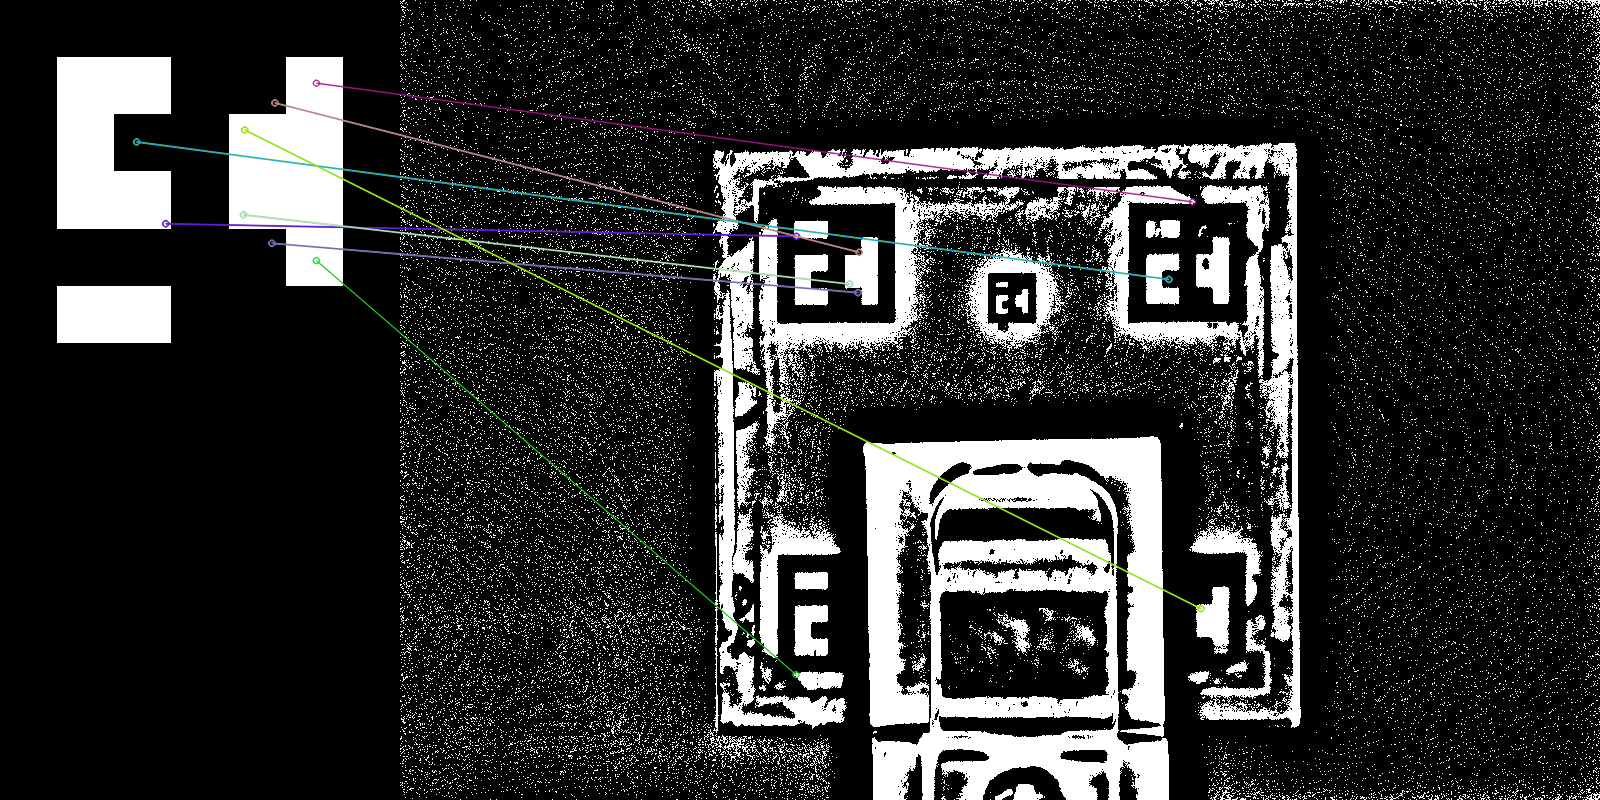
\includegraphics[width=0.9\textwidth]{image/classic_sift_matches}
  \label{fig:classic_sift_matches}
\end{figure}

\begin{figure}
  \caption{Detections of the marker middle using the \ac{SIFT} approach, using a sliding window and postprocessing}
  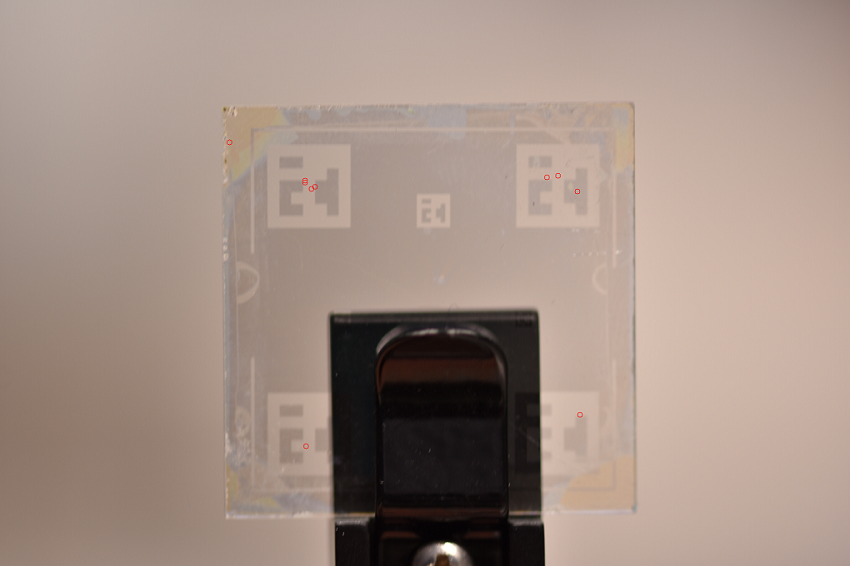
\includegraphics[width=0.7\textwidth]{image/classic_sift_final_matches}
  \label{fig:classic_sift_final_matches}
\end{figure}

\begin{figure}
  \caption{Adaptive thresholding on a image from the real test set}
  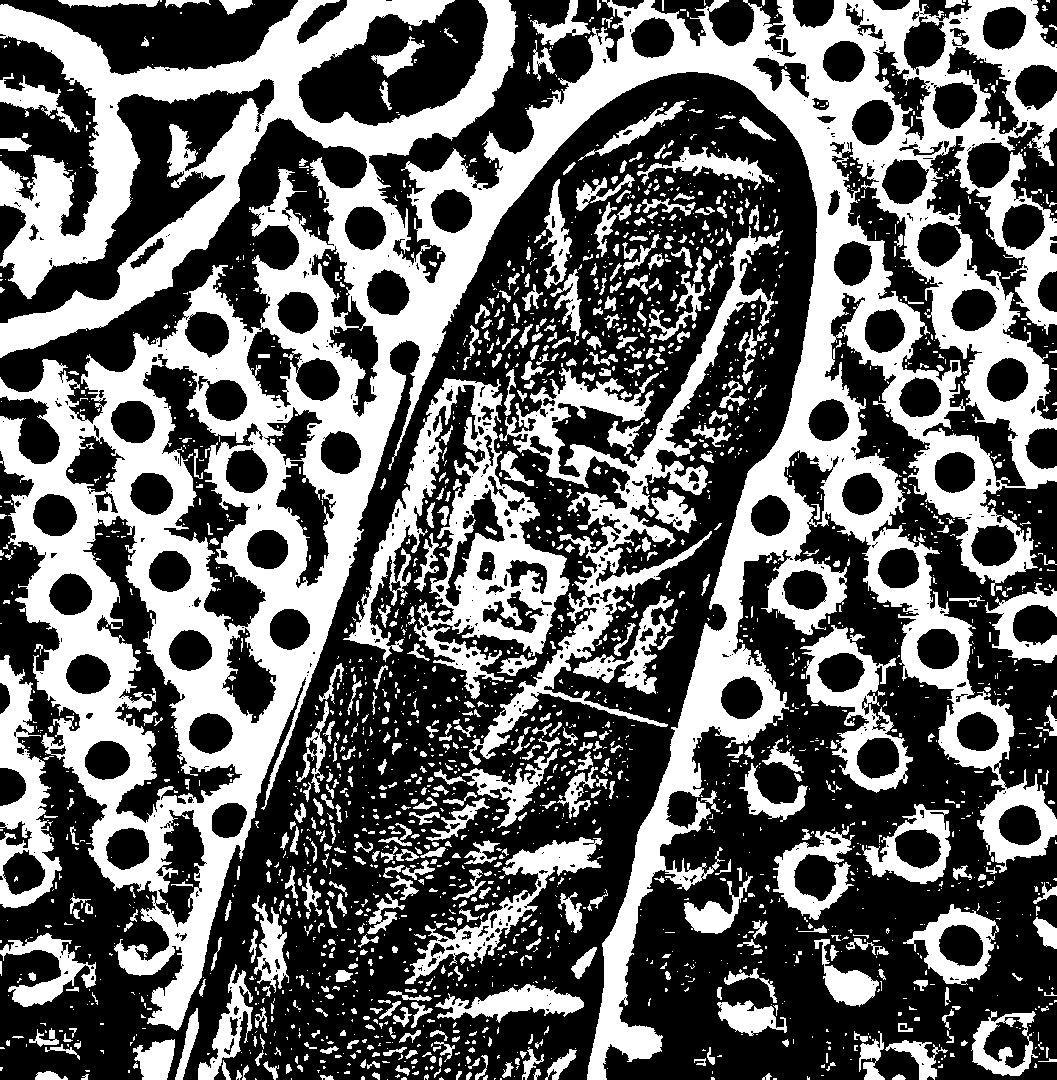
\includegraphics[width=0.4\textwidth]{image/classic_sift_thresh_on_finger}
  \label{fig:classic_sift_thresh_on_finger}
\end{figure}

Since the output of adaptive thresholding on the image in the histogram approach segments the parts of the \ac{ArUco} marker well, as seen in \autoref{fig:classic_sift_matches}, I also used a feature matcher on the thresholded image and a image of the \ac{ArUco} marker to detect the marker positions. Due to familiarity, I used \acp{OpenCV} implementation of \ac{SIFT} with the brute-force matcher for this task. Since feature matching in this way will separate its matches across the repeating marker structures, as seen in \autoref{fig:classic_sift_matches}, I applied a sliding window around the matching process. Finally the positions of the matches in the image are moved by the difference of their position in the marker image and the middle of the marker image to cluster them. The results of that process can be seen in \autoref{fig:classic_sift_final_matches}, where the majority of the matches land on or near the middle of a \ac{ArUco} marker in the image. However when using this matching process on an image of the real test set, nothing is detected, since the thresholded image there does not preserve the structure of the \ac{ArUco} marker, as seen in \autoref{fig:classic_sift_thresh_on_finger}.

\subsection{Conclusion}

While I cannot try out all combinations of data transformations and image algorithms to find the best \ac{ArUco} marker detection algorithm, these attempts do illustrate that finding a machine learning free detection algorithm for this task is a hard problem, which therefore constitutes the usage of neural networks for this usecase.

\section{Software Architecture}

Python has support for the structuring of script files into modules in which data can be primarily exchanged between components through function call arguments. However for this work I chose to structure the project as loose script files that exchange data primarily through the filesystem. The advantage in that approach is that all intermediate results of the script pipeline necessarily stay in the filesystem and can be used for validation later. Furthermore should there be an error in the execution of a script later in the pipeline, that script can easily be started again with adapted code and tested on the input data it failed on without having to run all previous steps, for example retraining a model.

\subsection{Data Pipeline Overview}

\begin{figure}
  \caption{Overview of the most important data structures and scripts of the data pipeline from raw data to a dataset, orange nodes stand for data and blue nodes stand for python scripts}
  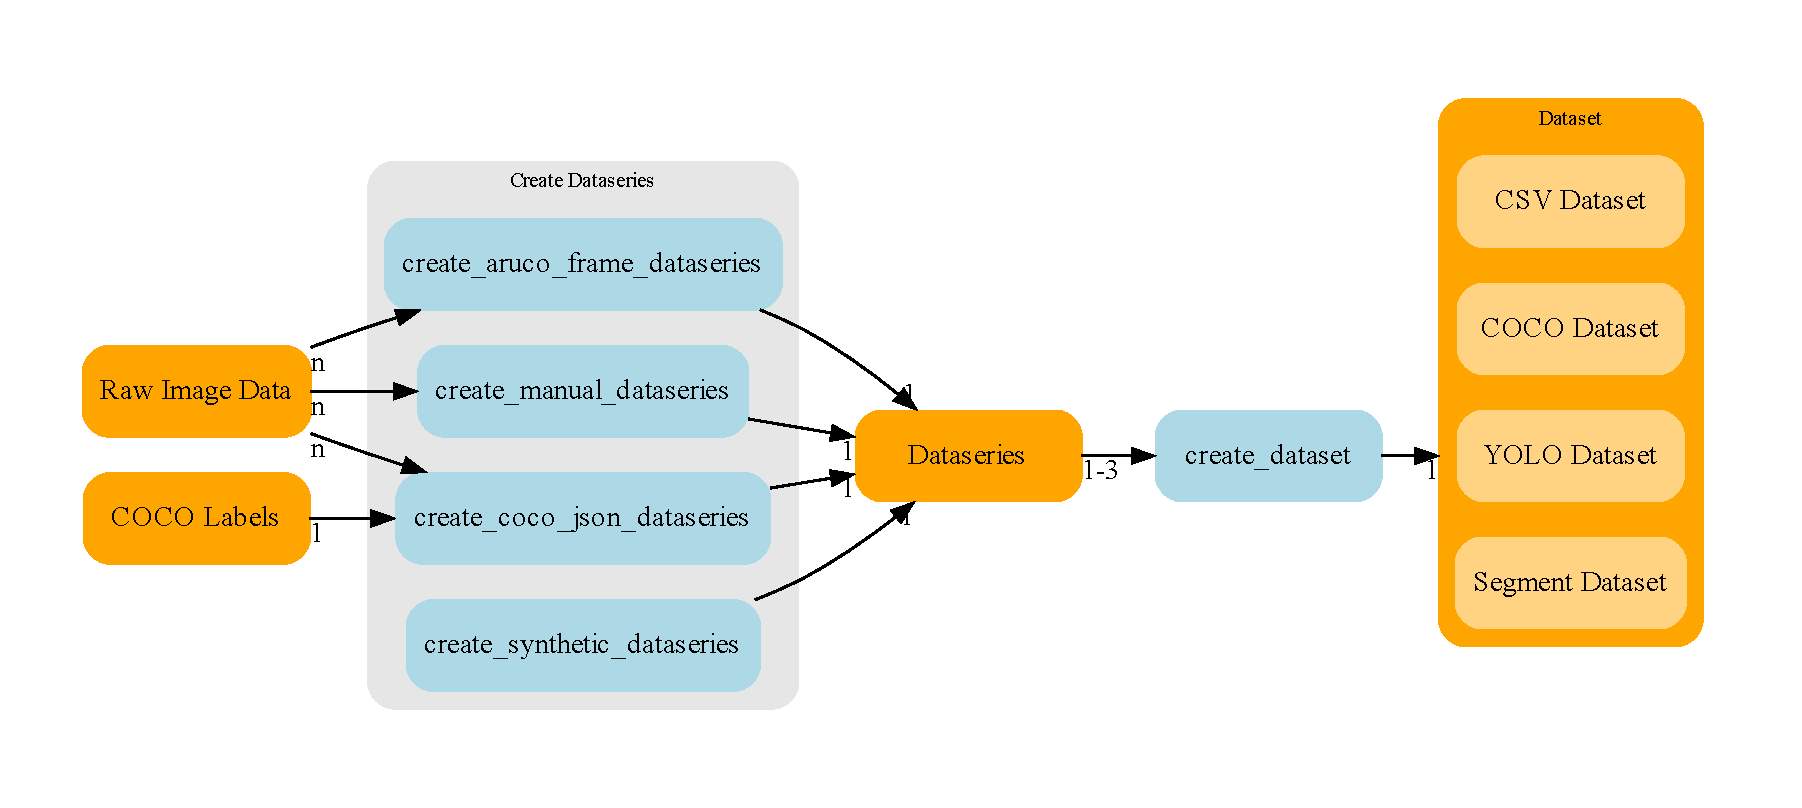
\includegraphics[width=\textwidth]{graph/arch_data}
  \label{fig:arch_data}
\end{figure}

The first part of the script pipeline serves four major goals. Firstly, it should define a standardized label data type, that all dataset types can be build from. Secondly, it should allow for a simple way to annotate large amounts of data to keep the labeling workload low. Thirdly, it should output a range of dataset types such that the data can be easily trained on many predefined \ac{NN} packages and projects to get the best results. Fourth, it should build augmentations into the data such that custom augmentations can be tested on different models without having to adapt the dataloader that comes with the model. Most predefined dataloaders and model backbones/heads share few data formats, making changes there difficult.

The overview seen in \figureref{fig:arch_data} shows the various dataset types, that are build by the \texttt{create\_dataset} script, addressing the third goal. The \texttt{create\_aruco\_frame\_dataseries} script, which is described in more detail in a later section, addresses the second goal. Furthermore augmentations are added in the \texttt{create\_dataset} script, addressing the fourth goal.

\subsection{Label Data Type}

\begin{figure}
  \centering
  \subcaptionbox{Unrotated image and polygon (orange) / bounding box (blue) labels}
     {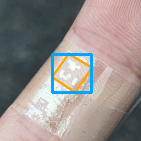
\includegraphics[width=0.3\textwidth]{image/polygon_pog_1}}
  \subcaptionbox{Image and polygon (orange) / bounding box (blue) labels after 50° rotation, as well as the old bounding box data in gray}
     {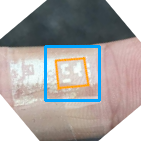
\includegraphics[width=0.3\textwidth]{image/polygon_pog_2}}
  \caption{Two images from the testset showing a polygon label in orange and a bounding box label in blue, after a rotation augmentation operation was applied in image two, the new bounding box label could only be created based on the old labels information, which was already too large since it could not capture the rotation of the object, the polygon label however can be augmented with the image without loosing label accuracy by transforming the polygon points.}
  \label{fig:polygon-good}
\end{figure}

Image augmentation libraries have support for many datatypes to accommodate for many usecases. However Albumentations only supports segmentation masks, bounding boxes and keypoints. While segmentation masks are a versatile data structure both bounding boxes and keypoints can be reduced to polygons. Furthermore polygons are able to more accurately fit to an objects structure during augmentations as seen in \figureref{fig:polygon-good}. Therefore I use polygons as labels in dataseries and throughout most of the \texttt{create\_dataset} script. Afterwards the bounds of the polygon's vertices can be used to transform it into a bounding box for object detection dataset types or the polygon can be rasterized to create a segmentation dataset.

\subsection{Train Pipeline Overview}

\begin{figure}
  \caption{Overview of the most important data structures and scripts of the training pipeline from datasets to \ac{mAP} scores, orange nodes stand for data and blue nodes stand for python scripts}
  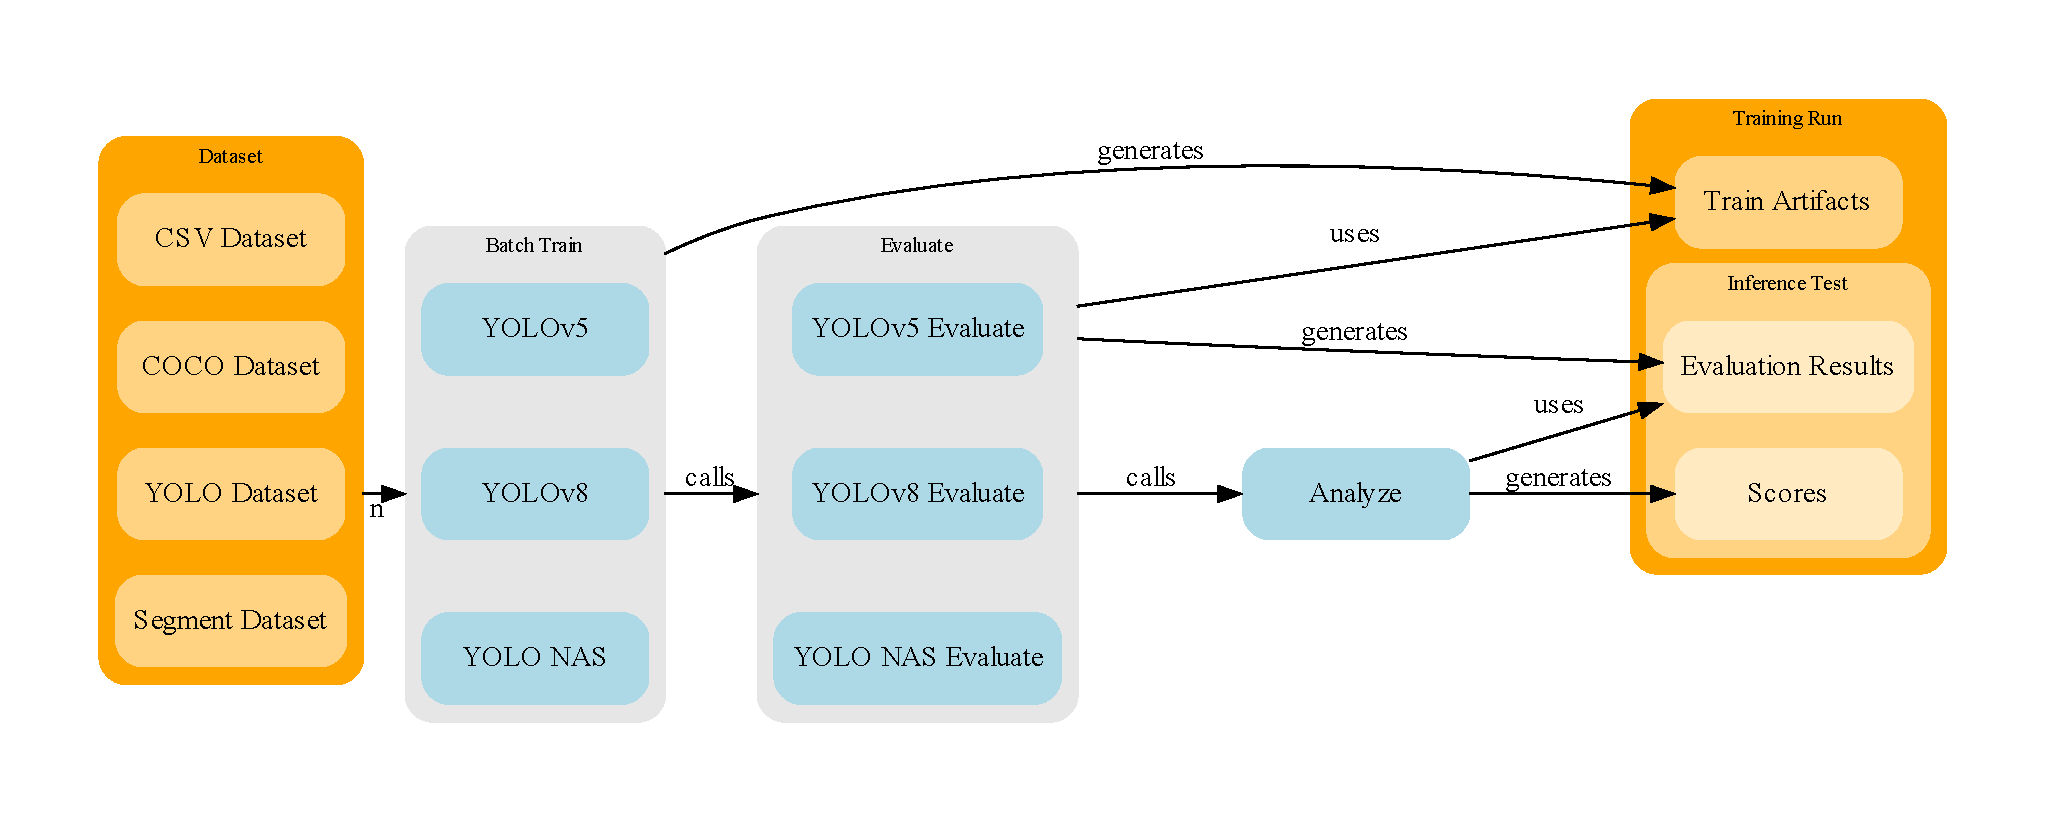
\includegraphics[width=\textwidth]{graph/arch_train}
  \label{fig:arch_train}
\end{figure}

As seen in \figureref{fig:arch_train} the training pipeline mainly consists of batch train, evaluate and analyze scripts. Batch train and evaluate scripts are implemented for each network source independently due to varying script usage and data formats. Batch train and evaluate scripts are split such that a model can be evaluated using a different set of inference parameters without retraining it. The analyze script implements the \ac{mAP} calculation and is split from the evaluate scripts since it can be implemented independently of each model source. Batch train scripts can take multiple datasets at once for an ensemble training run.

A training run folder contains the train artifacts, which refers to all files, including the model weights, that are created during training. The relation between training runs and inference tests was omitted in the figure, however training runs can contain multiple inference tests. Each inference test contains evaluation files which refers to a list of tuples of the networks predicted output and the target output in the xyxy bounding box format in addition to the confidence values, which can be used for the \ac{mAP} calculation, as well as extra files for validation. The scores consist of the calculated VOC 2007, VOC 2010 and COCO \ac{mAP} scores, as well as intermediate results of the calculation for validation.

\section{Automated Annotations}

\begin{figure}
  \centering
  \subcaptionbox{First marked image of a aruco frame dataseries}
     {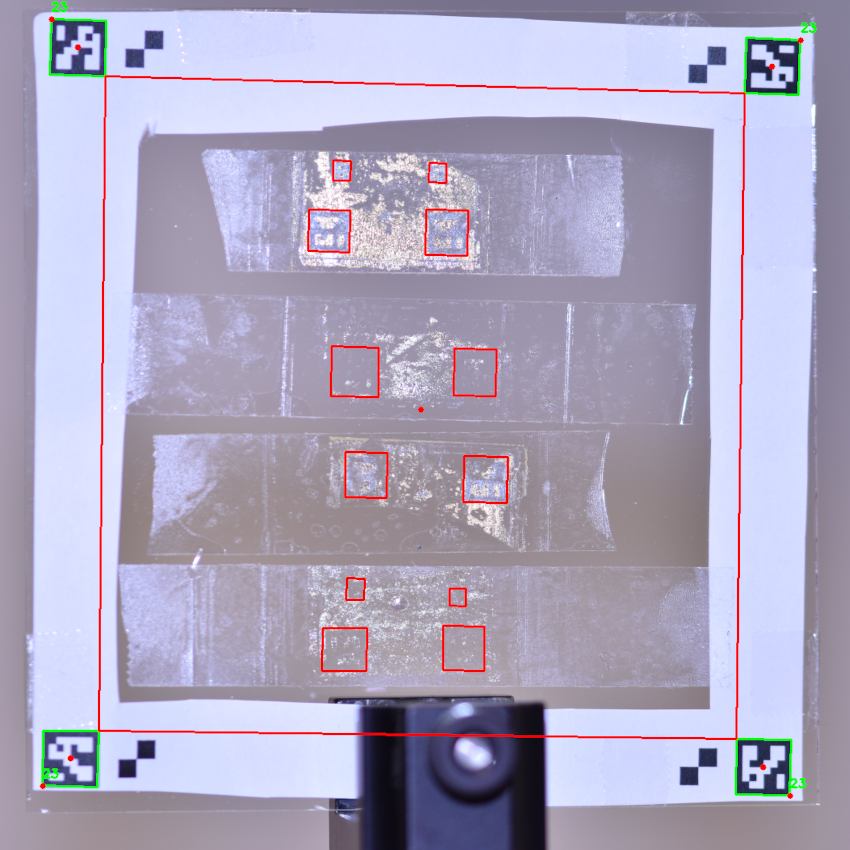
\includegraphics[width=0.45\textwidth]{image/af_markings_1}}
  \subcaptionbox{Later marked image of a aruco frame dataseries}
     {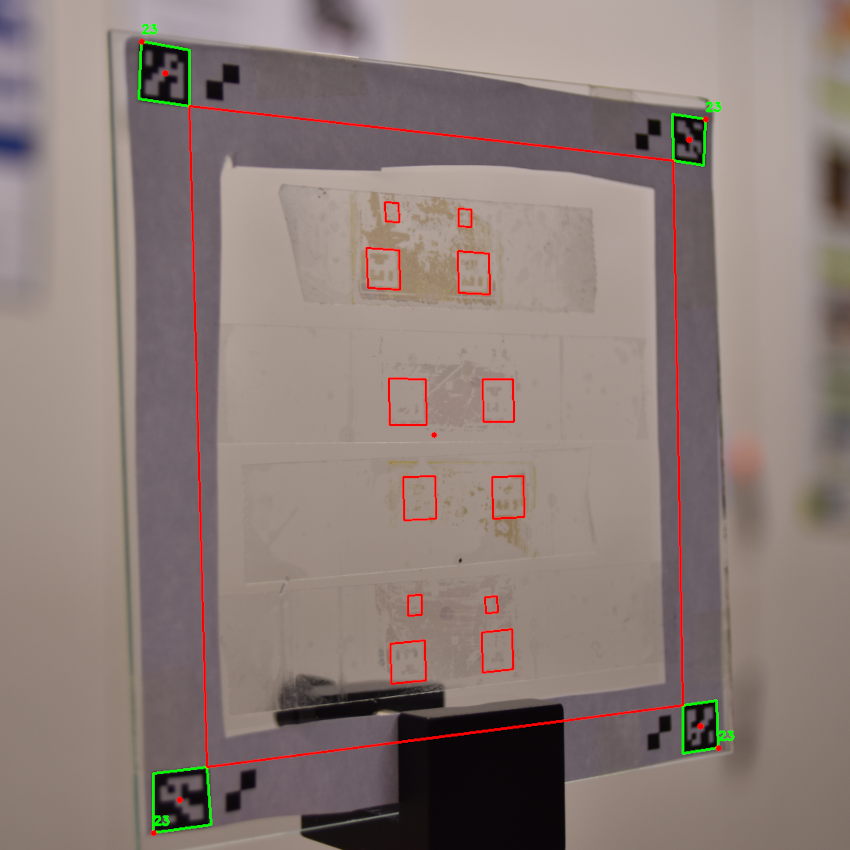
\includegraphics[width=0.45\textwidth]{image/af_markings_2}}
  \caption{Two example images from the validation data of the \texttt{create\_aruco\_frame\_dataseries} script.}
  \label{fig:af_markings}
\end{figure}

To make the annotation of training data faster we printed 4 \ac{ArUco} markers on the corners of a paper, cut out the middle and used it as a frame for the actual training data as seen in \figureref{fig:af_markings}. Since the tape containing the markers is on a planar surface, the position of the plane the markers sit on in 3D space within the images can be computed based on the \ac{OpenCV} detectable \ac{ArUco} markers on the paper corners. By manually labeling the first image in such a series of images, where the placement of the markers does not change, the positions of all the markers in the rest of the series can be inferred.

\begin{figure}
  \caption{Position of the \texttt{create\_aruco\_frame\_dataseries} script in the pipeline}
  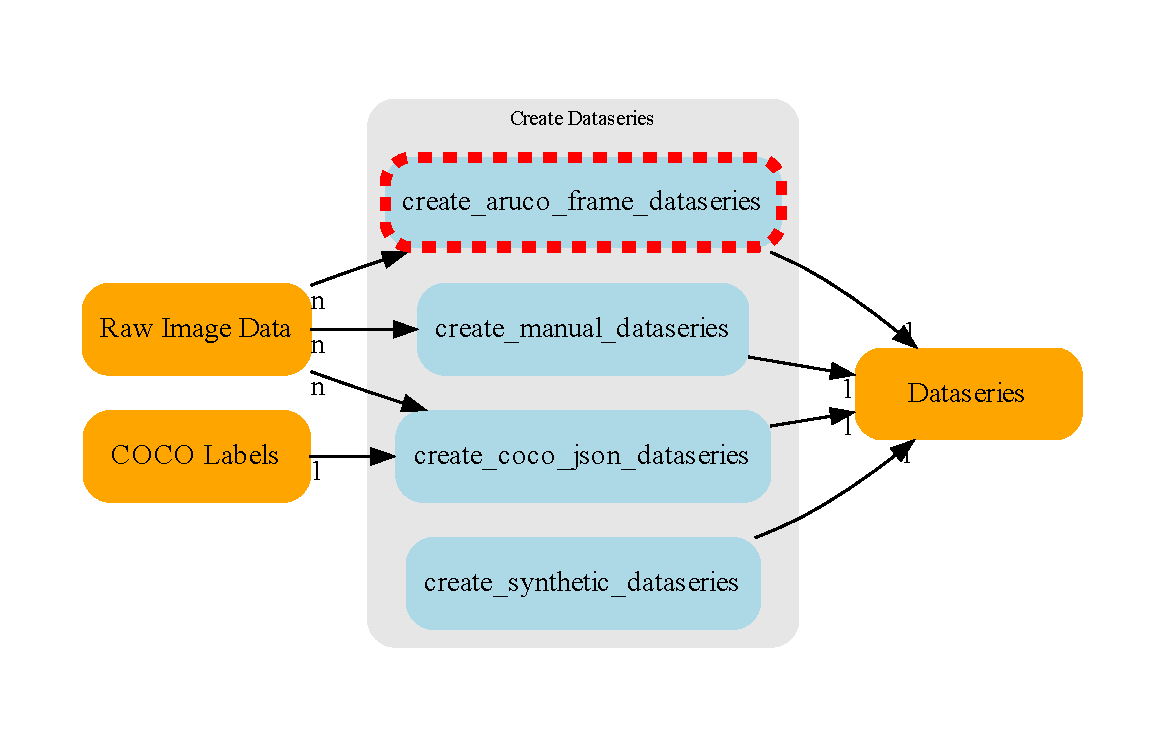
\includegraphics[width=0.65\textwidth]{graph/arch_data_af_focus}
  \label{fig:arch_data_af_focus}
\end{figure}

The position of this script within the pipeline can be seen in \figureref{fig:arch_data_af_focus}. After the script starts the first image of the image series given in the command line arguments is analyzed by the built-in \ac{OpenCV} \ac{ArUco} detector. Should there be 4 detected markers, the script will attempt to find the inner rectangle, which is the largest marked in red in \figureref{fig:af_markings}. For the Homography calculation in the next step it is important that the corners of the inner rectangle have a stable ordering. 

There are two algorithms for finding the inner rectangle. The first one, also called \texttt{legacy\_rect\_finding} in the script, sorts each markers corners that are the closest to the middle into a list based on the quadrant the marker is in the image. Therefore \texttt{legacy\_rect\_finding} works independent of the orientations of the markers on the paper frame, however it is dependant on the placement of the markers in the image. 

The second algorithm assumes that all \ac{ArUco} markers on the paper frame have the same orientation and sorts their corners closest to the image middle into the rect based on their index in the marker as seen in \autoref{lst:irf}. The relationship between the indices is visualized in \figureref{fig:inner_rect_indices}. As long as the assumptions of the two algorithms hold, they both result in a stable U-shaped ordering of the corners.

\begin{figure}
  \caption{Matching corner indices of the \ac{ArUco} rectangles and the red inner rectangle corners written on the image}
  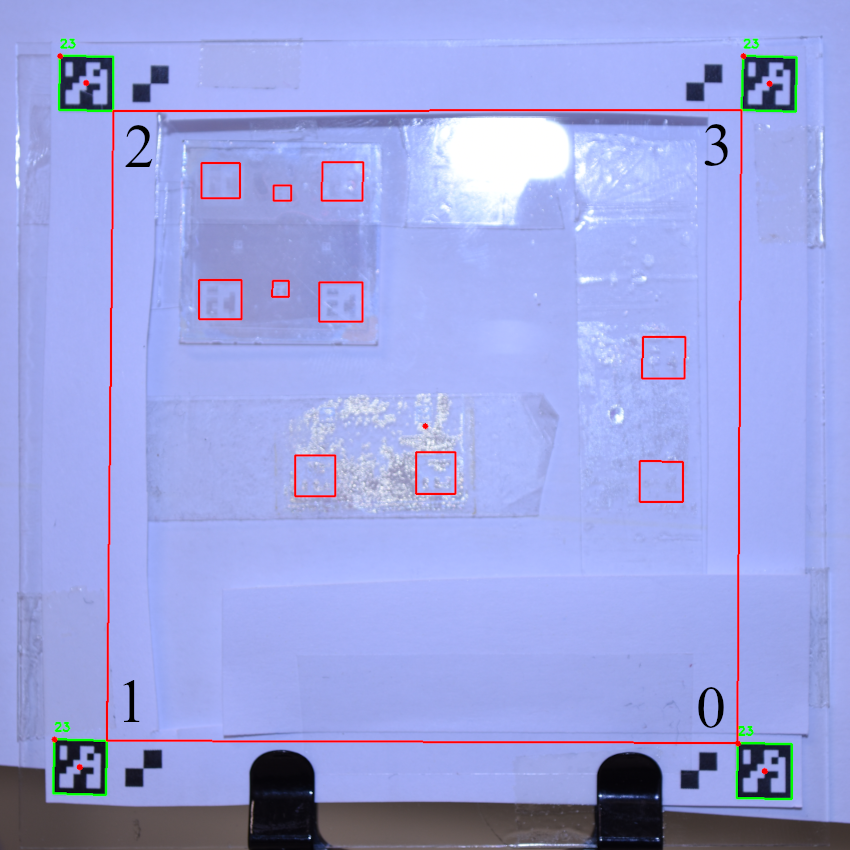
\includegraphics[width=0.5\textwidth]{image/af_markings_3}
  \label{fig:inner_rect_indices}
\end{figure}

\begin{code}
\captionof{listing}{Inner Rectangle Finding}
\label{lst:irf}
\begin{minted}{python}
  def find_inner_rect(each_arucos_corners, center):
    inner_rect = [None, None, None, None]

    for corners in each_arucos_corners:
        # Get index of closest corner to image center in aruco marker rectangle
        min_i, _ = min([(i, distance(v, center)) for i, v in enumerate(corners)], 
                       key=lambda x: x[1])
                
        # The markers corner closest to the middle is the min_i'th vertex of the inner rect
        min_vert = corners[min_i]
        inner_rect[min_i] = (int(min_vert[0]), int(min_vert[1]))
        
    return inner_rect
\end{minted}
\end{code}

Afterwards a homography from the inner rect corners to the points $(0,h), (0,0), (w,0), (w,h)$ is computed, the initial image is transformed using it and the user can label all visible markers on the transformed image in a \ac{OpenCV} \ac{GUI} window.

Once the user is done, the labels are transferred to each other image by finding the \ac{ArUco} frame like before, finding its inner rectangle, computing the homography for it and transforming the user defined labels as polygons onto the image using the user defined points and the two homographies. However this time the homography is computed from the points $(0,h), (0,0), (w,0), (w,h)$ to the inner rect corners.

\section{Augmentations}

This section describes the augmentations that were implemented into the \texttt{create\_dataset} script. They were implemented such that the chance of application and their strength can be set through the command line arguments. Furthermore the images are copied for augmentations such that the original not augmented training images and labels are kept in the dataset at least once. The position of the augmentations in the pipeline is shown in \autoref{fig:arch_data_aug_focus}.

\begin{figure}
  \caption{Position of augmentations in the pipeline}
  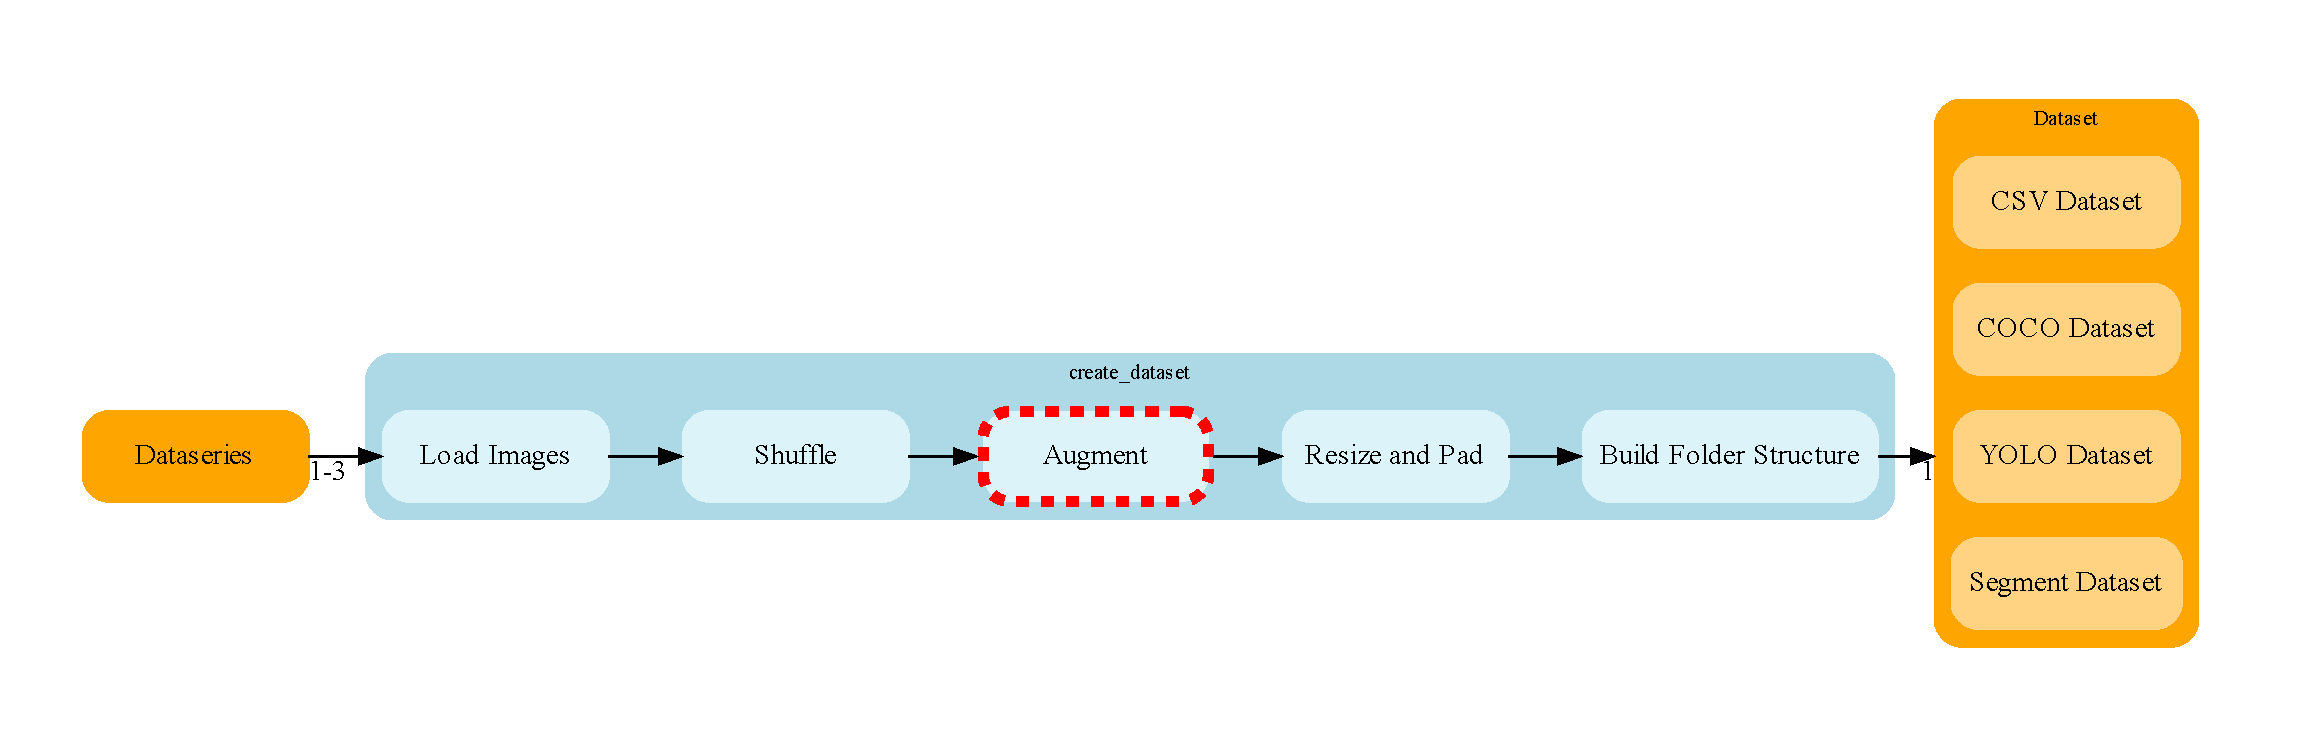
\includegraphics[width=\textwidth]{graph/arch_data_aug_focus}
  \label{fig:arch_data_aug_focus}
\end{figure}

\subsection{Smart Grid Shuffling}

The training data contains series of images with multiple tapes in the same relative positions on the glass plate. However these relative positions should not be learned, since the trained model should recognize single markers independently of their surroundings. 

One image augmentation that breaks up the overall image structure is grid shuffling. Albumentations already has an implementation for grid shuffling, however that implementation does not work on bounding boxes, since the grid lines, on which the image is split apart, may also split apart bounding boxes and the objects they describe. This makes sense for Albumentations, which is build to work within dataloaders as a fast augmentation pipeline. However in this case the speed of the augmentation does not matter as much, since it is build into the dataset before the training. To make grid shuffling work for this case, I adapted it to not split the image on a fixed grid but on gaps between polygon labels. To keep the algorithm simple, all cuts are axis aligned.

\subsubsection{Implementation}

The first part of smart grid shuffling traverses the polygon labels in order of their centroid position on a given axis. Should the distance between the bounding boxes of two polygons on the given axis be larger than a threshold, then the image is cut along the other axis and a segment is created, as seen in \autoref{lst:sgs_cut}.

% \begin{algorithm}
%   \SetAlgoLined
%   \KwIn{$I$: the image, $P$ the list of polygon label for the image, $D$ the axis to work in, $p$ the minimum distance between polygons for a cut}
%   \KwOut{$S$: list of segments}
%   $S \leftarrow []$ 

%   sort $P$ ascendingly based on polygon centroid position on axis $D$\;
%   \For{$i\gets0$ \KwTo len($P$)-2}{
%     $d \leftarrow$ distance between $P[i]$ and $P[i+1]$;

%     \uIf{$d$ > $p$}{
%       $e_{Last} \leftarrow S[-1]$.end;

%       $e \leftarrow$ $D$ component of midpoint in area between $P[i]$ and $P[i+1]$;


%     }
%   }
%   \caption{Segment generation part of smart grid shuffling}
% \end{algorithm}

% [caption={Smart Grid Shuffling Algorithm in Pseudocode},captionpos=b,label=lst:sgs_cut]

\begin{code}
\captionof{listing}{Cutting Part of Smart Grid Shuffling}
\label{lst:sgs_cut}
\begin{minted}{python}
# Generate image segments by cutting the image between polygon labels through x or y
def segment_img_between_poly_labels(
  img: Mat, polys: List[Polygon], 
  axis: Literal[0,1], 
  min_cut_distance = 5):

  segments = []
  
  # Sort the polygon labels on the axis they should be cut in, 0 for x and 1 for y
  polys = sort_polys_in(axis, polys)
  
  # Traverse the labels in order and generate image segments
  for i in range(len(polys)-1):
  axis_distance = distance_between_this_and_next_poly_on_axis(polys, i, axis)

    if axis_distance > min_cut_distance:

      # Get the segment cutting position on axis
      last_end = segments[-1]['end'] if len(segments) > 0 else 0
      end = mid_between_poly_ends(polys, i, axis)

      # Generate segment
      segment_polys = get_polys_in_segment(polys, last_end, end)
      segment_img = img[:, last_end:end] if axis == 0 else img[last_end:end, :]
      segments.append({
        'end': end,
        'polys': segment_polys,
        'img': segment_img,
      })

  # Generate last image segment analogously with end being the image size
  segments.append(last_segment)
  
  return segments
\end{minted}
\end{code}

The second part of smart grid shuffling defines the recombination of the image segments along an axis into a common image and a common label list as seen in \autoref{lst:sgs_comb}.

\begin{code}
\captionof{listing}{Segment Combination Part of Smart Grid Shuffling}
\label{lst:sgs_comb}
\begin{minted}{python}
def rebuild_img_from_segments(segments, target_img_size, axis: Literal[0,1]):
  result_img = get_empty_image_of_size(target_img_size)
  result_polys = []

  # Traverse image and place image segments
  pos = 0
  for seg in segments:
    if axis == 0: # x
      result_img[:,pos:seg['end']] = seg['img']
    else: # y
      result_img[pos:seg['end'],:] = seg['img']
        
    result_polys.append(seg['polys'])
    pos = seg['end']
    
  return aug_image, aug_polys
\end{minted}
\end{code}

The last part uses the defined segment cutting and recombination operations to first segment the image along the y-axis and shuffle the resulting segments. Each segment is then further segmented on the x-axis, shuffled and recombined. Finally all y-axis segments are recombined and returned.

\begin{code}
\captionof{listing}{Segment Combination Part of Smart Grid Shuffling}
\label{lst:sgs_main}
\begin{minted}{python}
# Main method
def smart_grid_shuffle(img, polys: List[Polygon], img_size_wh):

  # Segment in y first
  segments_y = segment_img_between_poly_labels(img, polys, 1)

  # Shuffle the resulting y-segments
  random.shuffle(segments_y)

  # Then segment all segments_y on the x axis
  for segment_y in segments_y:
    segments_x = segment_img_between_poly_labels(segment_y['img'], segment_y['polys'], 0)

    # Shuffle segments to change their position
    random.shuffle(segments_x)
    
    # Rebuild y-segment from x-segments
    segments_img, segments_polys = rebuild_img_from_segments(segments_x, segment_y.size(), 0)
    
    segment_y['img'] = segments_img
    segment_y['corners'] = segments_polys

  # Return recombined y-segments
  return rebuild_img_from_segments(segments_y, img_size, 1)
\end{minted}
\end{code}

\subsubsection{Example}

\begin{figure}
  \centering
  \subcaptionbox{Training image before augmentation}
     {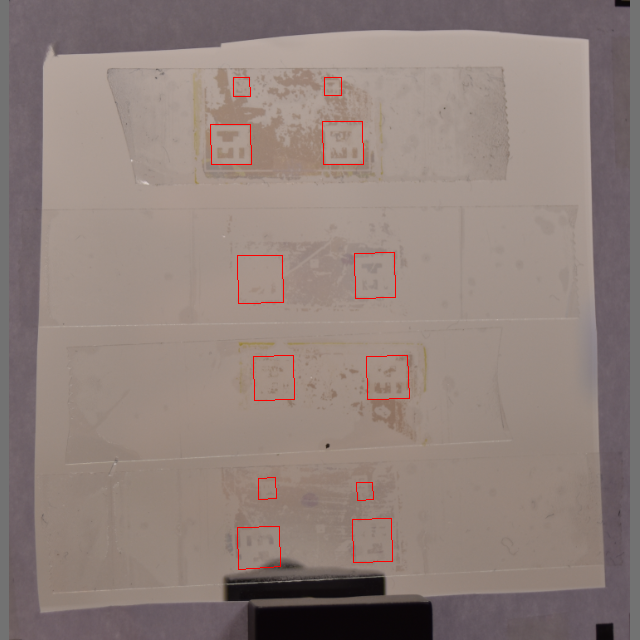
\includegraphics[width=0.45\textwidth]{image/aug_sgs_before}}
  \subcaptionbox{Training image after augmentation}
     {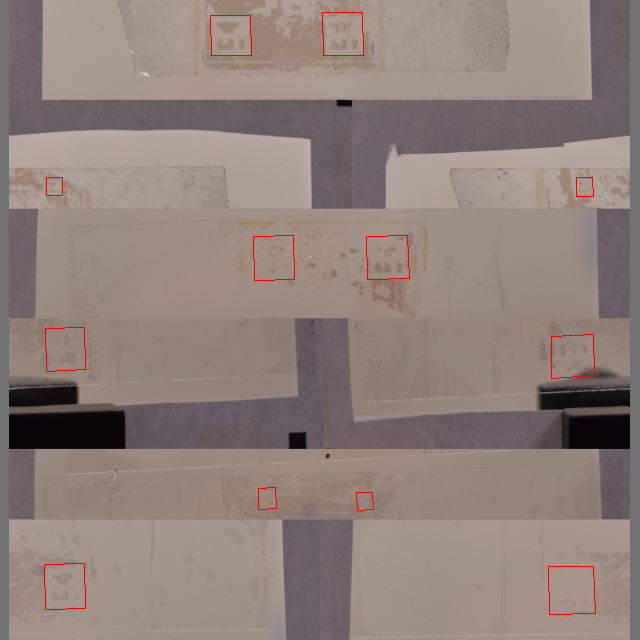
\includegraphics[width=0.45\textwidth]{image/aug_sgs_after}}
  \subcaptionbox{Training image before augmentation}
     {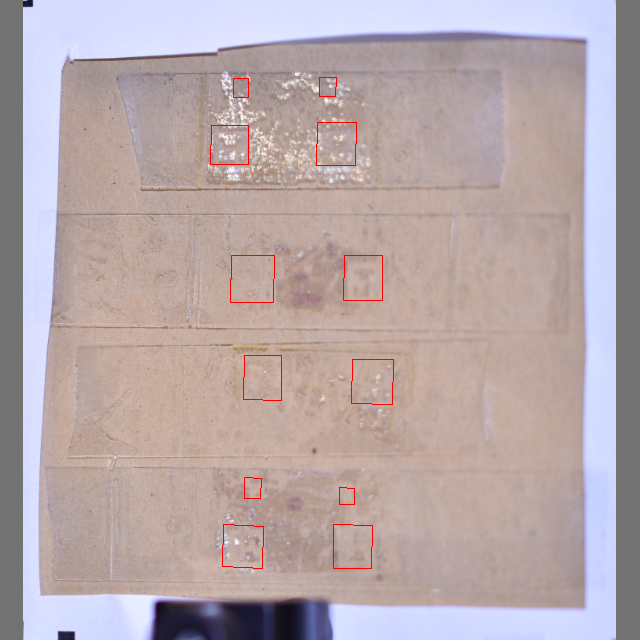
\includegraphics[width=0.45\textwidth]{image/aug_sgs_before2}}
  \subcaptionbox{Training image after augmentation}
     {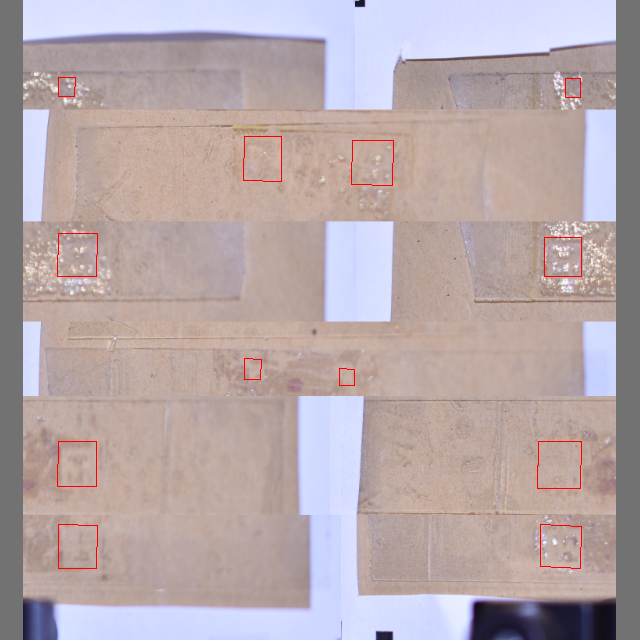
\includegraphics[width=0.45\textwidth]{image/aug_sgs_after2}}
  \caption{Two examples for smart grid shuffling with similar initial label arrangement}
  \label{fig:aug_sgs_example}
\end{figure}

The smart grid shuffling augmentation cuts and reassembles the image such that as much of the possibly important surrounding pixels of the polygon labels are preserved, but that still removes any reoccurring patterns in the image, in which the labels may be arranged by, as seen in \autoref{fig:aug_sgs_example}.

\subsection{Label Dropout}
\label{sec:aug_ld}

\begin{figure}
  \centering
  \subcaptionbox{Training Image before augmentation}
     {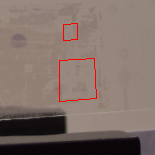
\includegraphics[width=0.45\textwidth]{image/aug_pld_before}}
  \subcaptionbox{Training Image after augmentation}
     {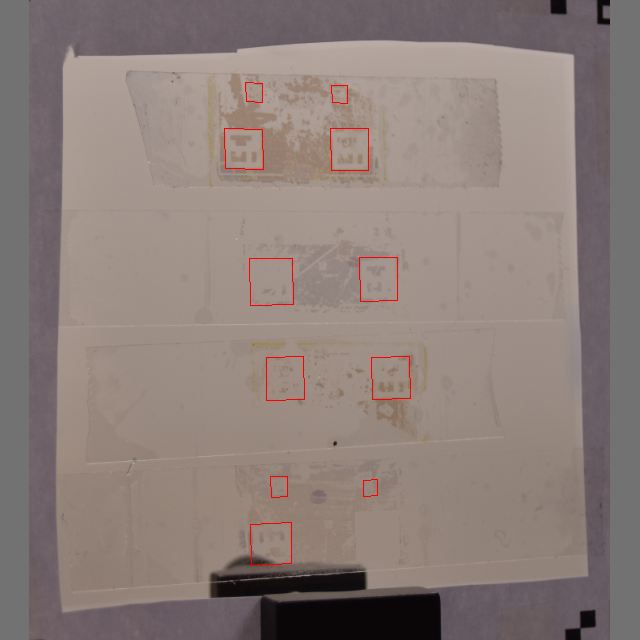
\includegraphics[width=0.45\textwidth]{image/aug_pld_after}}
  \caption{An example for label dropout}
  \label{fig:aug_pld_example}
\end{figure}

To further discourage the model from learning label arrangements in the image, the label dropout augmentation randomly chooses a label, removes the label from the image and removes the label entry. The label is removed from the image by taking its polygon, scaling it around its centroid by 1.2 and rasterizing the result on the image using the color on the image at the polygons centroid position. The result of that operation can be seen in \autoref{fig:aug_pld_example}.

\subsection{Homogeneous Matrix Transform}

The rotation and perspective transformations are both combined into a homogeneous matrix transform step to prevent code duplication and to improve performance, since this step requires postprocessing.

For most augmentations there is a chance setting and possibly a strength setting depending on the augmentation. Here the chance for a rotation of 90 degree multiples is combined with the chance of rotation of any angle, the maximum rotation angle, the chance for perspective transform and the maximum perspective transformation strength. Firstly all settings are build into two transformation matrices and both are combined. Then the resulting matrix is used to transform the image as well as the polygon label vertices, as seen in \autoref{fig:aug_mat_example}.

\begin{figure}
  \centering
  \subcaptionbox{Training Image before augmentation}
     {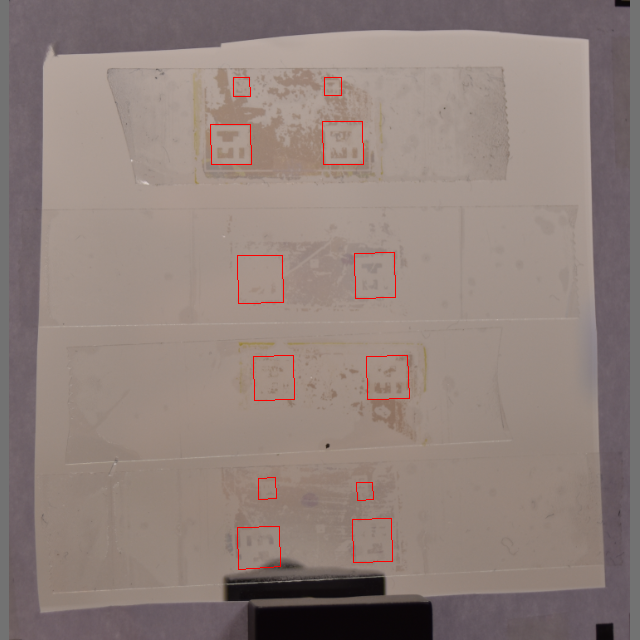
\includegraphics[width=0.45\textwidth]{image/aug_mat_before}}
  \subcaptionbox{Training Image after augmentation}
     {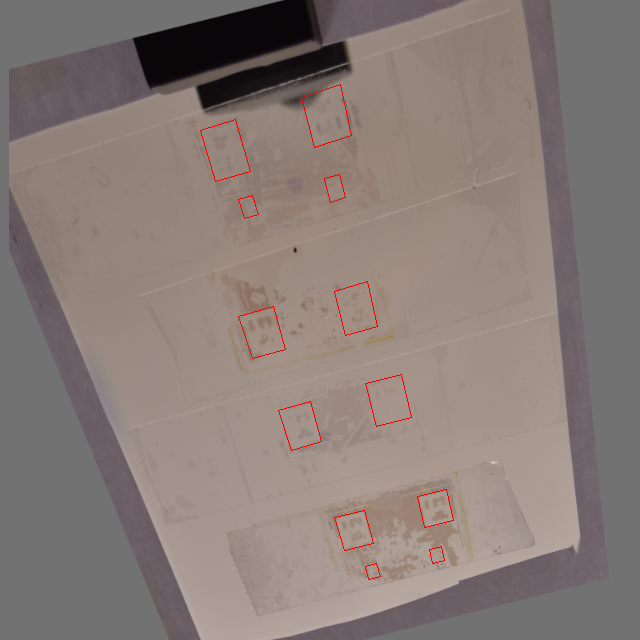
\includegraphics[width=0.45\textwidth]{image/aug_mat_after}}
  \caption{An example for matrix transform augmentation}
  \label{fig:aug_mat_example}
\end{figure}

\subsubsection{Out of Bounds Cases}
\label{sec:oob}

After the transformation cases of \ac{OOB} labels have to be handled, as labels may be rotated out of the visible image area. I defined a minimum visibility threshold at 60\%, since many labels can be hard to see even if the whole label is in the image in the training data. To compute visibility, first the intersection of the label polygon and the image bounds polygon is computed using Shapely. Visibility is then defined as the area of the intersection polygon divided by the area of the original label polygon. This computation is similar to the \ac{IoU} definition or to albumentations visibility calculation on bounding boxes\footnote{\url{https://albumentations.ai/docs/getting_started/bounding_boxes_augmentation/}, accessed on 05.11.2023}. Should the resulting visibility be lower than the threshold, the label entry is discarded from the list of label entries of the image and the remaining area, where the label was, is painted over as described in \autoref{sec:aug_ld}. Should it pass the visibility check but still intersect with the image border, the label is set to be the intersection from earlier, effectively clipping it within the image space.

\subsection{Random Crop}

\begin{figure}
  \centering
  \subcaptionbox{Training Image before augmentation}
     {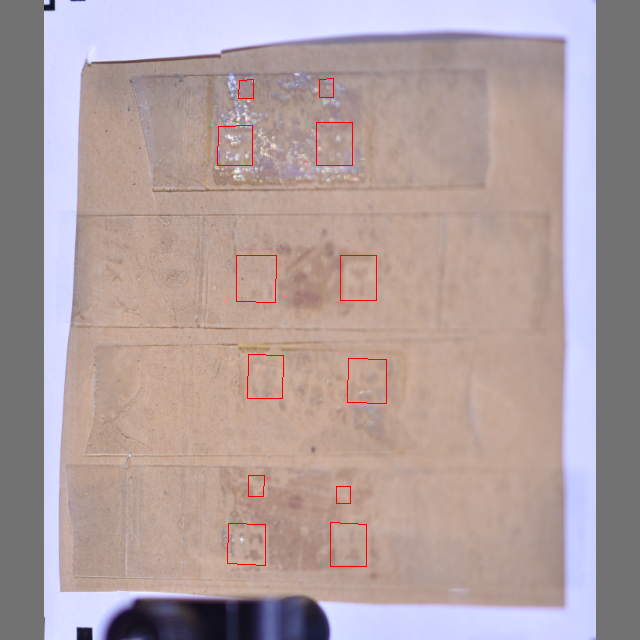
\includegraphics[width=0.45\textwidth]{image/aug_rc_before}}
  \subcaptionbox{Training Image after augmentation}
     {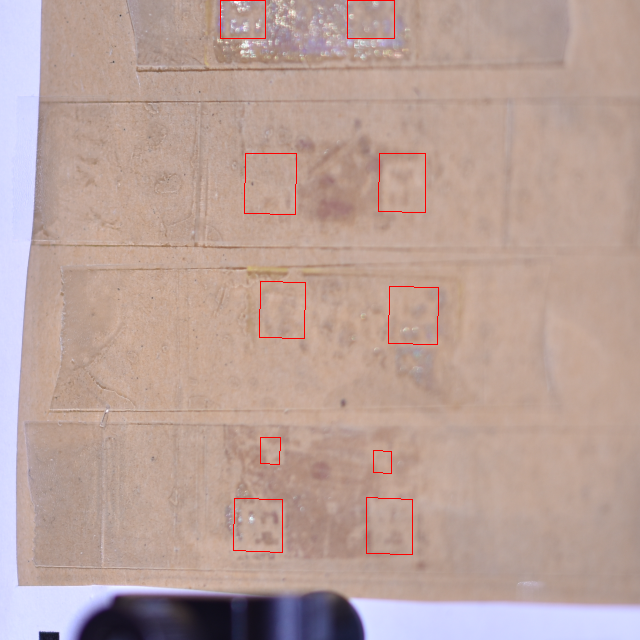
\includegraphics[width=0.45\textwidth]{image/aug_rc_after}}
  \caption{An example for random crop}
  \label{fig:aug_rc_example}
\end{figure}

The pipeline implements a random crop which crops a area of the datasets target image size out of the input image and moves the labels accordingly as seen in \figureref{fig:aug_rc_example}. Since this augmentation can also leave labels out of bounds the same procedure is applied on the resulting labels as described in \autoref{sec:oob}.

\subsubsection{Augmentation Versions}

\begin{figure}
  \centering
  \subcaptionbox{Training Image before augmentation}
     {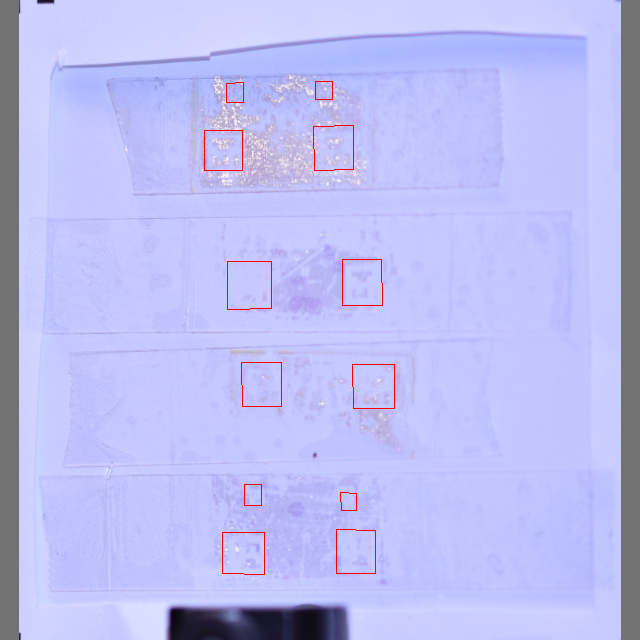
\includegraphics[width=0.45\textwidth]{image/aug_rc2_before}}
  \subcaptionbox{Training Image after augmentation}
     {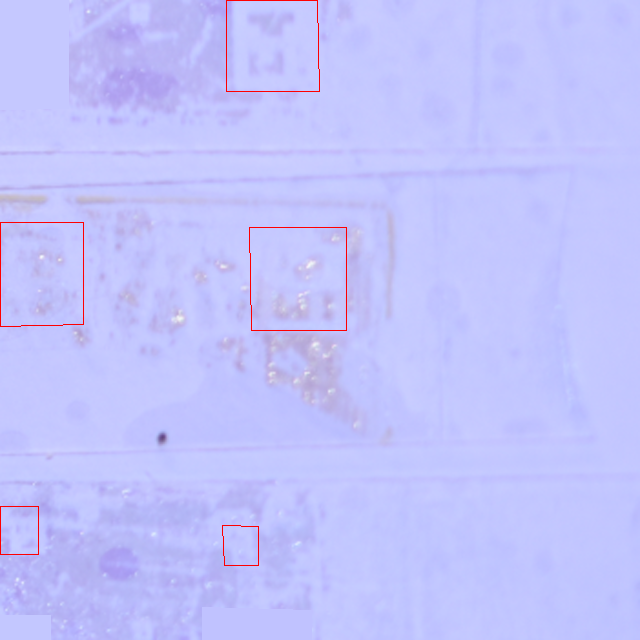
\includegraphics[width=0.45\textwidth]{image/aug_rc2_after}}
  \caption{An example for random crop v2, also showing on the borders of image (b) how out of bounds labels, that do not pass the visibility check, are overdrawn such that the residue of the marker on the image, that is without label, does not introduce a false negative into the training data, as described in \autoref{sec:oob}.}
  \label{fig:aug_rc2_example}
\end{figure}

The data pipeline also builds \ac{JSON} files into the dataset folder to make the whole dataset build process retraceable. Because of that, I did not change augmentations meaningfully, besides bug fixes once they were implemented, such that the \ac{JSON} files stay as backwards compatible as possible. In this case I also built a random crop, which crops an area of variable size out of the source image and then rescales that cropped part to the target image size, which is therefore implemented as its own augmentation: random crop v2. Examples for random crop v2 can be seen in \figureref{fig:aug_rc2_example}. Splitting the augmentations in versions this way also has the advantage, that the following evaluation can detect how much better a new version of an augmentation performs or if there is regression.

\subsection{Label Move}

\begin{figure}
  \centering
  \subcaptionbox{Training Image before augmentation}
     {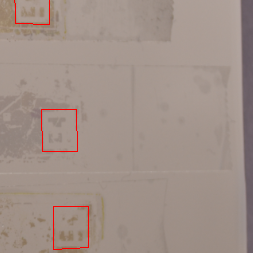
\includegraphics[width=0.45\textwidth]{image/aug_lm_before}}
  \subcaptionbox{Training Image after augmentation}
     {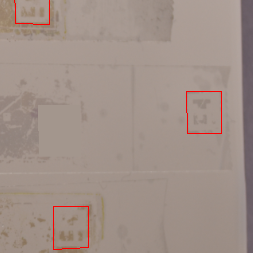
\includegraphics[width=0.45\textwidth]{image/aug_lm_after}}
  \caption{An example for label move}
  \label{fig:aug_lm_example}
\end{figure}

Label move works similar to label dropout as described in \autoref{sec:aug_ld}. However after removing the label from the image it is reinserted at a different place including the image structure, that the label describes, as seen in \autoref{fig:aug_lm_example}. 

Since inserting of images into other images in OpenCV works by copying slices only \ac{AABB} areas can be inserted at once. However when reinserting the labels image structure at another position, only the \ac{ArUco} marker structure should be inserted and not the surrounding image content. Therefore before inserting the labels image structure back, a mask is applied to it. That mask is just the labels polygon rasterized in white onto a black image. Using the mask as weights, the labels image structure is then reinserted.

\subsubsection{Label Move v2}

\begin{figure}
  \centering
  \subcaptionbox{Training Image before augmentation}
     {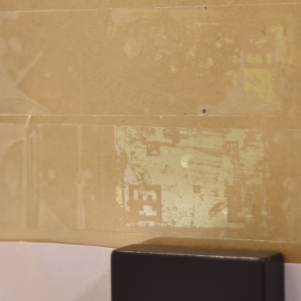
\includegraphics[width=0.45\textwidth]{image/aug_lm2_before}}
  \subcaptionbox{Training Image after label move augmentation}
     {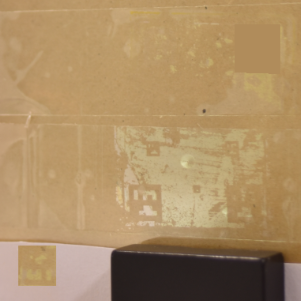
\includegraphics[width=0.45\textwidth]{image/aug_lm2_after_old}}
  \subcaptionbox{Training Image after label move v2 augmentation}
     {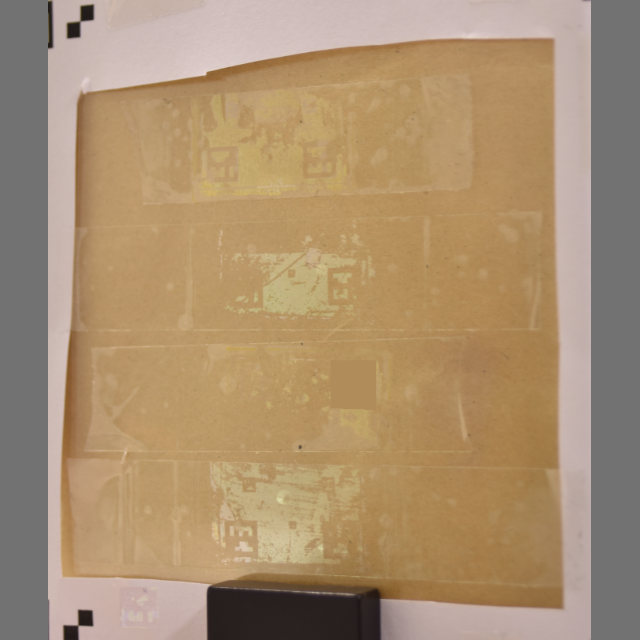
\includegraphics[width=0.45\textwidth]{image/aug_lm2_after}}
  \caption{An example for label move v2, in which the label is moved from the middle to the bottom left and despite the background color differences is not as noticeable, label borders are not drawn here to make the border differences of the augmentations more visible}
  \label{fig:aug_lm2_example}
\end{figure}

In the second version of label move has two additions to the operations of label move. 

Firstly the color of the labels image structure is roughly adapted to the target positions color. For this both the average RGB values of the image target area slice and the average RGB values of the labels image structure are computed. Then each pixel of the labels image structure is recolored based on the difference of the average RGB values before it is reinserted into the image.

Secondly gaussian blur is applied to the mask, which is a rasterized version of the labels polygon. Due to this change, the inserted labels image structure does not have strong contours anymore and gets a small color transition at its borders.

These changes help make the reinserted label look more natural in the new spot, as seen in \autoref{fig:aug_lm2_example}.

\subsection{Black Dot}

\begin{figure}
  \centering
  \subcaptionbox{Training Image before augmentation}
     {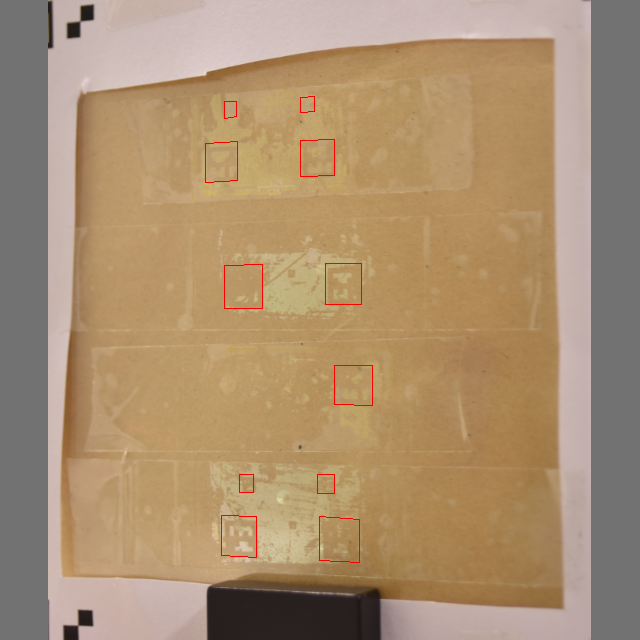
\includegraphics[width=0.45\textwidth]{image/aug_bd_before}}
  \subcaptionbox{Training Image after augmentation}
     {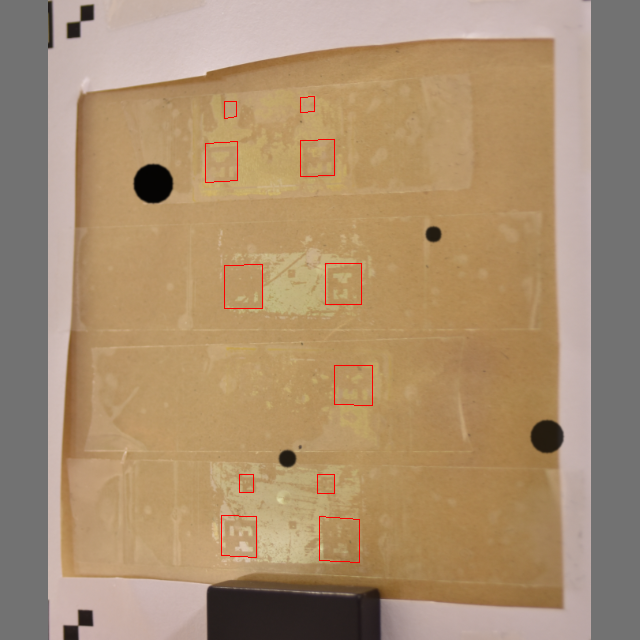
\includegraphics[width=0.45\textwidth]{image/aug_bd_after}}
  \caption{An example for black dot augmentation}
  \label{fig:aug_bd_example}
\end{figure}

A reoccurring issue with the application of \ac{SAHI}, which is discussed in more detail later, is, that dark objects in the test data were repeatedly and with large confidence misidentified as markers. To make sure that the network learns that dark areas in the image are not markers, I added an augmentation which adds black dots on parts of the image where no marker is. 

After the augmentation is started at least one black dot is added. Afterwards there is a 40\% chance that another black dot is added. If another black dot is added there is another 40\% chance for one more marker. This could continue forever, however it gets more and more unlikely to go on after each iteration. 

The insertion of black dots works similarly to label move, with the difference that a completely black image is inserted and that the mask is a circle. Furthermore like in label move v2, the mask is blurred using gaussian blur to create a color transition.

An example of black dot aug can be seen in \autoref{fig:aug_bd_example}.

\subsection{Label Curving}

\begin{figure}
  \centering
  \subcaptionbox{Training Image before augmentation}
     {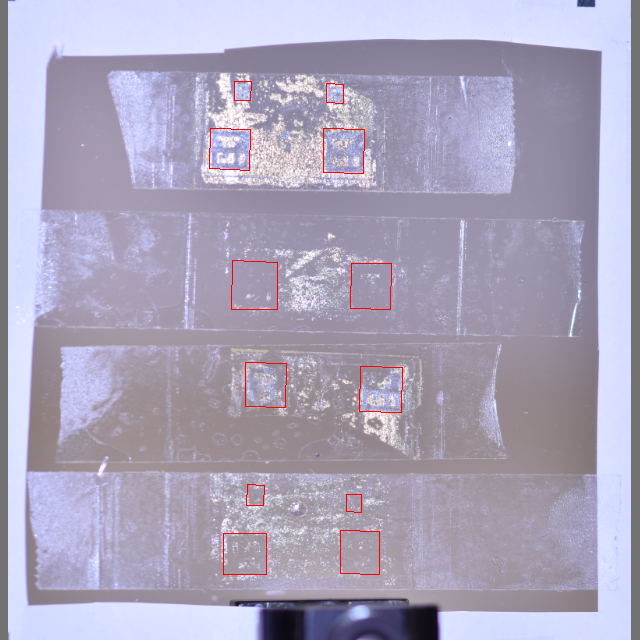
\includegraphics[width=0.45\textwidth]{image/aug_lc_before}}
  \subcaptionbox{Training Image after augmentation}
     {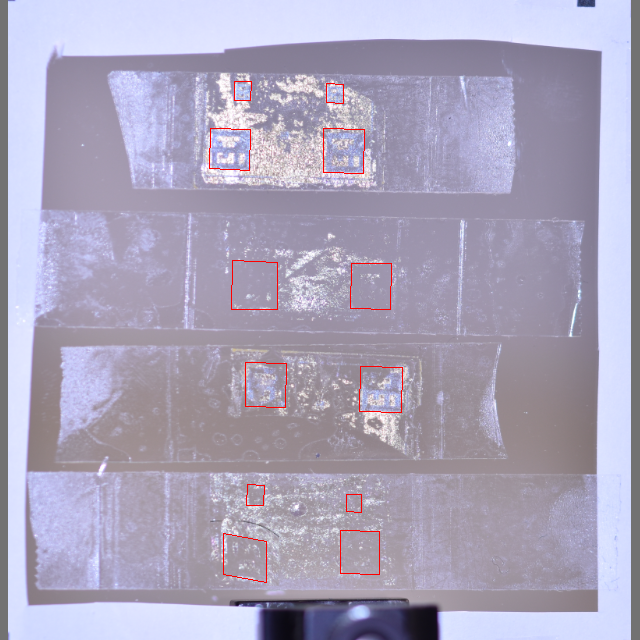
\includegraphics[width=0.45\textwidth]{image/aug_lc_after}}
  \caption{An example for label curving augmentation on the marker in the bottom left}
  \label{fig:aug_lc_example}
\end{figure}

Another reoccurrence in the test data was that the tape with the markers was rolled around a finger. Due to the nature of the training data, this case is currently not included in the fitting process. The label curving augmentation should therefore mimic the curved labels.

This augmentation again works similar to label move. However in this case the label is not moved anywhere. It is cut out and modified using \acp{OpenCV} \texttt{remap} function. \texttt{remap} takes, besides other parameters, two arrays, which represent the x and y coordinates each pixel should be mapped to. In this case the x coordinates stay the same but the y coordinates are mapped based on a half circle function to mimic the pixel displacement on a curved surface. The middle and the width of the half circle are randomly chosen. Alongside the image cutout the label vertices are also transformed, such that the label is still located over the image structure. However the polygon cannot fully capture the curving without new vertices, but since the polygons are transformed into bounding boxes in most cases this is not a problem. An example of label curving can be seen in \autoref{fig:aug_lc_example}.

\subsection{Gaussian Noise}

While augmentations that work with labels needed to be implemented specifically for this pipeline due to the label datatype. Pixel level augmentations are already defined and work just as well here. The gaussian noise augmentation here therefore works using the Albumentations gaussian noise transformation\footnote{\url{https://albumentations.ai/docs/api\_reference/augmentations/transforms/\#albumentations.augmentations.transforms.GaussNoise}, accessed on 06.11.2023}. 

Gaussian noise adds noise to each pixel in the image, with the strength of the noise being given by the normal distribution. Here gaussian noise is used to make sure to get a different result from similar training runs, such that the quality of a training run can be assessed.

% TODO?: \section{Synthetic Data}

\section{Inference}

\begin{figure}
  \caption{Position of evaluation inference in the pipeline}
  \includegraphics[width=0.75\textwidth]{graph/arch_train_eval_focus}
  \label{fig:arch_train_eval_focus}
\end{figure}

The inference on test data using previously trained models happens in the evaluation scripts, as shown in \autoref{fig:arch_train_eval_focus}. The inference can be optimized using additional filters and other techniques. One such technique is \ac{SAHI}. However since each type of model has its own evaluate script, because each type of model works slightly differently, certain techniques have to be implemented separately. Therefore \ac{SAHI} is currently not supported for \ac{YOLO}-NAS within this project.

\subsection{Bounding Box Filters}

Furthermore the bounding boxes from the inference results can be filtered independently of the model they come from. The application of \ac{SAHI} can result in an increased amount of false detections along the border of the image. To prevent this the size of a border along the the image bounds can be set and all bounding box predictions that fall within this border are filtered out. Additionally to filter predictions which are not square enough, which the \ac{ArUco} marker usually are not, a minimum squareness can be set. Squareness is here defined as $$ 
s(w,h)=
\begin{dcases}
    \frac{w}{h}, & \text{if } w\leq h\\
    \frac{h}{w}, & \text{otherwise}
\end{dcases} $$ where $w$ refers to the bounding boxes width and $h$ to its height. Due to the definition, the squareness score always lies between 0 and 1.

\subsection{Foreground Mask}

Since markers in the images are usually part of the foreground, a pretrained foreground segmentation network could help improve the detection scores.
To test this, I added support for masking of bounding box predictions. Since this is just for testing, this is not implemented fully into the pipeline. For the bounding box filtering, the area of the bounding box is cut out of the mask image and the maximum pixel value of the area is checked against a minimum threshold. Using the average instead of the maximum pixel value lead the lower scores.

\subsection{Fusion Inference}

The \texttt{fusion\_inference} script combines the predictions of multiple finished training runs as a post processing step. In comparison to \ac{SAHI}, \texttt{fusion\_inference} combines the output of the whole image from different fitted models is into one prediction, while \ac{SAHI} combines predictions on parts of the image from the same fitted model. During fusion inference, the bounding boxes are combined using the weighted boxes fusion approach from Solovyev et al. \cite{solovyev2021weighted}.

% TODO?: \section{Plotting}

\section{Automated Ensembles}

Given a set of dataseries as base and parameters for dataset creation, training and inference, the entire process for ensemble learning can now be automated. Furthermore, by starting multiple batch train instances and giving each information about its worker index and the total worker count, the training load on multiple datasets can be split among multiple \acp{GPU}. Finally, given a consistent naming scheme, the score results of the training runs can also be automatically plotted.

The top level scripts necessary for this are currently only implemented to work with the \ac{MIP} server structure, but could be ported to any \ac{GPU} server with Docker support.

\section{Hyperparameter Optimization}
\label{sec:hyper_opt}

To find an optimal combination of augmentations from the implemented ones, a hyperparameter optimization is implemented using Hyperopt. More precisely the search space for this usage of Hyperopt contains the chances for each augment to be applied on an image during dataset generation. Furthermore the strengths of augments that define one, such as the maximum rotation angle for the rotation augment, are also part of the search space. The epochs that should be trained for are also part of the search space. Since the validation data in the datasets used here can be similar to the training data, the hyperparameter optimization, which unlike the training runs on the test data, can then choose an earlier stopping point for the training, if further training does not increase the score further or in other words would overfit on the validation data. Finally the random seed for the dataset creation is also part of the search space, such that the best training run during the optimization is fully reproducible.

\section{Point Detection}

This section describes the development of the second part of the inference. After the areas of interest were found by the model which works on the whole image, this part finds the corner points of the marker within that area of interest.

\subsection{Point Head Approach}

For this approach I mainly used a MobileNetV2 as base, since this part should also be lightweight, and added custom head layers to the network architecture. For testing of larger models I also tested a VGG16 \ac{CNN} as the base network architecture. The custom head outputs eight numbers which are interpreted as the x- and y-coordinates of the 4 corners points of the marker. I tested different head architectures, such as a fully convolutional head, a two linear layer head and a three linear layer head.

The training dataloader for this approach uses a albumentations augmentation pipeline for the images and keypoints label. The augmentations used include image shifting, rotation, scaling and perspective effects, as well as changes in brightness, contrast, hue and saturation, to simulate different situations in real world data.

The learn rate used here starts at $0.001$ and decays every $100$ epochs by a factor $0.2$. 

% \begin{figure}
%   \centering
%   \subcaptionbox{Predictions on validation data}
%      {\includegraphics[width=0.2\textwidth]{image/pet_val_no_rot}}
%   \subcaptionbox{Predictions on rotated validation data}
%      {\includegraphics[width=0.2\textwidth]{image/pet_val_rot}}
%   \caption{Example of keypoint detection output with and without rotated validation data}
%   \label{fig:pet_rot_example}
% \end{figure}

The loss used here is Sinkhorn loss from the geomloss library \cite{feydy2019interpolating}, which unlike the standard loss for keypoint detection, \ac{MSE}, works with any permutation of points, removing the requirement of getting the right point order from the network. 
% The outputs predicted the position of markers in the validation data well. However the markers in the validation data were all almost axis aligned and had little rotation. When adding a rotation augmentation to the validation data, the weaknesses of the network become visible, as it fails to predict different rotations of the \ac{ArUco} marker, as seen in \autoref{fig:pet_rot_example}. Using a larger model, such as VGG16, as the base did not meaningfully improve the results.

\subsection{Segmentation Approach}

\begin{figure}
  \centering
  \subcaptionbox{Validation data}
     {\includegraphics[width=0.2\textwidth]{image/segpet_1_in}}
  \subcaptionbox{Predictions on validation data}
     {\includegraphics[width=0.2\textwidth]{image/segpet_1_pred}}
  \subcaptionbox{Validation data}
     {\includegraphics[width=0.2\textwidth]{image/segpet_3_in}}
  \subcaptionbox{Predictions on validation data}
     {\includegraphics[width=0.2\textwidth]{image/segpet_3_pred}}
  \caption{Examples of segmentation approach output}
  \label{fig:segpet_preds_example}
\end{figure}

As an alternative I also tested a U-Net. Except for changing the loss to dice loss for the segmentation masks, the rest of the approach stayed the same. The same albumentations augmentations used above also work on segmentation masks. However it is worth noting that the MobileNetV2 with a custom head has a total number of of $3,153,776$ parameters and therefore a parameter size of 12.03 \acp{MB}. The used here instead uses a total number of $44,034,081$ parameters and a parameter size of 167.98 \acp{MB}. It is therefore almost 14 times larger. Furthermore there is extra logic required for interpreting the segmentation mask. 
%Nonetheless, the prediction results of rotated markers fit closer to the marker corners even after rotation, as seen in \autoref{fig:segpet_preds_example}. 
Examples for the U-Net output on validation data can be seen in \autoref{fig:segpet_preds_example}. 

\subsubsection{Harris Corner Based Mask Interpretation}

\begin{figure}
  \centering
  \subcaptionbox{Harris Corner Ouput}
     {\includegraphics[width=0.2\textwidth]{image/segpet_mask_8_pred_corners}}
  \subcaptionbox{Rectangle prediction on the input image}
     {\includegraphics[width=0.2\textwidth]{image/segpet_mask_8_pred_rect}}
  \subcaptionbox{Harris Corner Ouput}
     {\includegraphics[width=0.2\textwidth]{image/segpet_mask_10_pred_corners}}
  \subcaptionbox{Rectangle prediction on the input image}
     {\includegraphics[width=0.2\textwidth]{image/segpet_mask_10_pred_rect}}
  \subcaptionbox{Harris Corner Ouput}
     {\includegraphics[width=0.2\textwidth]{image/segpet_mask_6_pred_corners}}
  \subcaptionbox{Rectangle prediction on the input image}
     {\includegraphics[width=0.2\textwidth]{image/segpet_mask_6_pred_rect}}
  \caption{Examples of the segmentation mask interpretation output}
  \label{fig:segpet_rect_interp}
\end{figure}

Using the output of \acp{OpenCV} implementation of Harris corner detector, each triplet of corner points is considered as a candidate for the marker. Each point triplet $A,B,C$ is scored based on the dot product between $\overline{BA}$ and $\overline{BC}$, the length ratio of $\overline{BA}$ and $\overline{BC}$ and finally the length of $\overline{BA}$ and $\overline{BC}$. After the largest and most rectangle like triplet of points has been found, the last point of the rectangle is computed as follows: $D = A + \overline{BC}$, completing the marker rectangle points $A,B,C,D$, as seen in \autoref{fig:segpet_rect_interp}. 

It is worth noting, that using point triplets and predicting the last point comes with the disadvantage of perspective transformed markers not being detected correctly, since in that case $\overline{BC}$ and $\overline{AD}$ are not the same. However using three points improves the stability, since a whole corner may be misidentified in the segmentation mask.

% TODO: Point mapping accuracy in good/bad cases and show one good and one bad case 
% For eval: 75% of point order assessments correct

\subsubsection{Hough Transform Based Mask Interpretation}

\begin{figure}
  \centering
  \subcaptionbox{Harris corner ouput}
     {\includegraphics[width=0.2\textwidth]{image/segpet_mask_2_pred_corners}}
  \subcaptionbox{Rectangle prediction based on Harris corners}
     {\includegraphics[width=0.2\textwidth]{image/segpet_mask_2_pred_rect}}
  \subcaptionbox{Hough transform output lines and line intersections}
     {\includegraphics[width=0.2\textwidth]{image/segpet_mask_2_pred_intersects}}
  \subcaptionbox{Rectangle prediction based on line intersections}
     {\includegraphics[width=0.2\textwidth]{image/segpet_mask_2_lines_pred_rect}}
  \caption{Example of improved mask interpretation using Hough transform}
  \label{fig:segpet_lines_improvement}
\end{figure}

The \acp{OpenCV} implementation of Hough transform results in predicted lines on the mask edges. These lines are then lengthened such that the span the image and intersection points of these lines are computed. These intersection points are then used as in the harris corner approach. The advantage of using line intersections is that, if multiple corners of the mask are not clearly defined, all 4 corners of the marker can still be predicted as seen in \autoref{fig:segpet_lines_improvement}. % TODO: Found hough parameters manually trough heuristic

\subsection{Point Sorting}

\begin{figure}
  \caption{Pixel comparisons between the \ac{ArUco} marker image and the thresholded image snippet}
  \includegraphics[width=0.4\textwidth]{image/pet_point_sorting_compare}
  \label{fig:pet_point_sorting_compare}
\end{figure}

For now the different approaches only output points. However to detect how the marker lies in 3D space, it is also necessary to sort the points based on the rotation of the marker. For this, the input image is thresholded using \acp{OpenCV} adaptive threshold implementation. Afterwards a homography is computed to map the given rectangle in the image onto another image. Finally, using pixel comparisons each 90 degree rotation of the projected and thresholded image is tested against the \ac{ArUco} marker, as seen in \autoref{fig:pet_point_sorting_compare}. The rotation which is the closest fit for the marker is then chosen and the points are ordered accordingly.

\chapter{Evaluation}
\label{chap:eval}

This chapter covers the results of the training and hyperparameter search, as well as the data used for training.

\section{Data}

I got batches of images for the training and test data over the course of the time I was working on the thesis. In total I received 261 images with an \ac{ArUco} frame and 118 of tapes directly on skin at the time of writing. 

\subsection{Training Data}

Of the images, that were meant for training data and work with the \texttt{create\_aruco\_frame\_dataseries} script, I manually filtered the images for ones, on which I could recognize at least the majority of the markers, such that the training data is not too diluted. During development I build more and more dataseries from these batches of images and refined old dataseries. I then named datasets that use specific sets of these dataseries \texttt{gpv1}, \texttt{gpv2} and \texttt{gpv3}, for the version and the folder called \texttt{good pics} I filtered usable images into. \texttt{gpv1} datasets are build from 67 images, \texttt{gpv2} datasets from 35 images and \texttt{gpv3} datasets from 140 images. For the creation of the \texttt{gpv3} set I visited the material science department of the Kiel University and could take a glass plate with marker tapes home. I then combined dataseries from \texttt{gpv2} with a new dataseries from images we took at the material science department and a dataseries from 67 images I took with my phone at home of the glass plate to create \texttt{gpv3}.

During dataset creation a set percentage of images and their labels are randomly chosen as the validation data for the dataset and therefore the validation data also comes from the aforementioned dataseries.

\subsection{Test Data}

From the 118 images of tapes directly on skin I used 55 good ones to build the third version of the test data. There were concerns, that choosing fitted models based on their \ac{mAP} score on the test set would lead to overfitting. At the same time I wanted to test against images that were close to the real world use case. Therefore the test set was split into two sets, one for evaluation in ensemble runs and for hyperparameter search and one for a final test at the end. The test sets were split manually, but such that the score of a model tested on a previous version test set was similar in both sets, and such that both sets contain a variety of hand poses, that are at the same time not so similar that overfitting on one set would lead to a good score on the other. Since some pairs of the 55 original test images were similar, a random split would have been prone to putting images that are too similar in the ensemble and in the final test set, such that both would not have been different enough. This split then resulted in a 25 image ensemble test set and a 30 image final test set.

The third version of the test data was labeled using makesense.ai\footnote{\url{https://www.makesense.ai}, accessed on 11.11.2023} for better accuracy than the \texttt{create\_manual\_dataseries} script, which currently lacks a zoom feature. The labels were exported as polygons in the \ac{COCO} \ac{JSON} format, were then converted to a dataseries using the \texttt{create\_coco\_json\_dataseries} script and finally build into a dataset.

While I had the glass plate with marker tapes on it at home, removing the tapes from any surface carries a risk of damaging the marker structure on the tapes. Since the machine that creates the marker tapes was broken for most of the time I worked on this thesis, I did not want to risk breaking the few good tapes that we had and therefore could not build more test data on my own.

\section{Human Testing}

To get a score that I can compare the evaluation results to, I gathered scores that humans would achieve on this detection task. To do this, I distributed the images of the final test set and a instructions paper on the Kiel University WeTalk instance and Discord. The instructions paper contains a general introduction to the task, a perfect example marker, example training images with labels and step by step instructions for the labeling process. The labeling was done on makesense.ai\footnote{\url{https://www.makesense.ai}, accessed on 11.11.2023}, since it does not require an installation and instead works in the browser, while also containing all nessecary tools and, since the dataset is small enough to be distributed directly as files. In total there were 7 participants who returned their marked labels. For the evaluation I treated the resulting label data the same as the network output and generated \ac{mAP} scores using the same scripts. The resulting \ac{mAP} scores can be seen in \autoref{tab:human_test_result}.

\begin{table}
  \begin{tabular}{ c c c }
   & Pascal VOC 2010 \ac{mAP} & COCO \ac{mAP} \\ 
   \hline
   Best Result & 84.37\% & 46.52\% \\
   Average Result & 75.41\% & 37.58\% \\
   \hline
  \end{tabular}
  \caption{\label{tab:human_test_result}Results of human labeling accuracy tests}
\end{table}

\section{Testing Scope}

In this section I describe some of the fixed parameters during the testing. Since this work introduces many variables, such as model type, augmentation parameters and model specific hyperparameters, some of them need to be fixed to keep the scope simple enough. These constraints are based on earlier and smaller scale tests.

\subsection{Model}

After the implementation of the \ac{YOLO}v8 models into the training and testing pipeline, using the \ac{YOLO}v8 models instead of \ac{YOLO}v5 models did not increase the test scores on initial tests. \ac{YOLO}-NAS-S only achieved a \ac{mAP} score of 4\% on initial tests and 6\% after two built in augmentations were disabled.

The models were compared using their default parameters. For \ac{YOLO}v5, these were the parameters defined in the built in \texttt{hyp.scratch-low.yaml}. For \ac{YOLO}v8, these were the default parameters of the \texttt{ultralytics} packages \texttt{model.train()} function. For \ac{YOLO}-NAS-S, these were the hyperparameters stored in the \texttt{roboflow\_yolo\_nas\_s.yaml}.

The preprint of the paper from Treven et al. \cite{terven2023comprehensive} was released after most of the implementation for this work was already done. It also contains a comparison of \ac{YOLO} models, but one on the \ac{COCO} dataset. In this comparison the top three models were \ac{YOLO}v7, which achieved a score of 56.8\%, Scaled-\ac{YOLO}v4, which achieved a score of 56.0\% and \ac{YOLO}v5, which achieved a score of 55.8\%. However \ac{YOLO}v8 and \ac{YOLO}-NAS only got a score of 53.9\% and 52.2\% respectively. This does not explain the especially low scores of \ac{YOLO}-NAS-S, but it does validate the lower \ac{YOLO}v8 results.

Due to these results, and since smaller models can be used on more devices, most testing was done on \ac{YOLO}v5s.

\subsection{Dataset}

During initial testing of the datasets using yolov5s as the model to train, there was an increase in \ac{mAP} score from the bigger \texttt{gpv1} dataset to the smaller \texttt{gpv2} dataset, where more samples where sorted out based on image quality. However, while the scores without augmentation further increased with the dataset version, for \texttt{gpv3} the maximum scores did not increase. While the stagnation of scores can also stem from a combination of augmentations that were not suitable for \texttt{gpv3}, I mainly kept testing with \texttt{gpv2} instead, such that newer tests would be better comparable with older tests. The results can be seen in \autoref{fig:initial_dataset_compare}. % TODO: redo this with newer runs?

\begin{figure}
  \caption{Results of initial comparison of datasets on yolov5s, with built in yolov5 augmentations enabled and using two manually defined sets of augmentations \texttt{def} and \texttt{def2}, as well as runs without dataset augmentation, with 9 configurations and 5 runs per configurations for a total of 45 training runs}
  \includegraphics[width=\textwidth]{image/yolov5s-dataset-compare}
  \label{fig:initial_dataset_compare}
\end{figure}

\subsection{Inference}

Of the available inference parameters I mainly used \ac{SAHI} in the tests, since the markers in the testset were small and \ac{SAHI} increased the \ac{mAP} score in initial tests, or none.

\section{Augmenting from Zero} % TODO: Did I talk about randomness in training runs for ensembles anywhere?
\label{sec:aug_ens_zero}

As a test for the usefulness of the added augmentations, I ramped up the usage rates of an augmentation from 0\% to 100\% in 10 steps and did five training runs per step for a total of 50 training runs per augmentation. Using more training runs per configuration would make the values here more accurate, but would also take longer and use more electricity. The results shown here can therefore not be perfectly accurate, but give an idea of how the usage of an augmentation generally changes the scores.

\subsection{Smart Grid Shuffle}

Without the application of \ac{SAHI} a slight uplift in scores is visible throughout the plot, as seen in \autoref{fig:zero_sgs_plot}. Furthermore the correlation between the chance of augmentation usage and the \ac{mAP} score values of the training runs is 43\% for the VOC 2010 \ac{mAP} score and 52\% for COCO, showing that there is a moderate positive correlation.

\begin{figure}
  \caption{Results of Smart Grid Shuffle ensemble run without \ac{SAHI}}
  \includegraphics[width=\textwidth]{image/zero-based-sgs-ensemble-2-thesis}
  \label{fig:zero_sgs_plot}
\end{figure}

With \ac{SAHI} all scores increase, as seen in \autoref{fig:zero_sgs_sahi_plot}. Furthermore improvements flatten out earlier and stagnate after 10\% of usage chance.

\begin{figure}
  \caption{Results of Smart Grid Shuffle ensemble run with \ac{SAHI}}
  \includegraphics[width=\textwidth]{image/zero-based-sgs-sahi-ensemble-2-thesis}
  \label{fig:zero_sgs_sahi_plot}
\end{figure}

\subsection{Rotation}

The rotation augmentation is the one which improved the scores the most, as seen in \autoref{fig:zero_rot_plot}. The correlation for the VOC 2010 score is 54\% and for the COCO score is 21\% here. This may indicate that the precise placement of the bounding boxes suffers in the cases, where the marker could be easily detected before when using more rotation augmentation. However at this stage in development my biggest focus is to detect more markers, so the VOC 2010 score has more weight.

\begin{figure}
  \caption{Results of Rotation ensemble run without \ac{SAHI}}
  \includegraphics[width=\textwidth]{image/zero-based-rot-ensemble-2-thesis}
  \label{fig:zero_rot_plot}
\end{figure}

% TODO: Add sahi plot

\subsection{Random Crop v2}

Random Crop v2 had the worst impact on scores, as seen in \autoref{fig:zero_rc2_plot}. The correlation for the VOC 2010 score here is -43\% and for COCO is -30\%. This may be, because it zooms too far into the image and such large markers do not appear in the test set. Default Random Crop did not show similar impact on the scores.

\begin{figure}
  \caption{Results of Random Crop v2 ensemble run without \ac{SAHI}}
  \includegraphics[width=\textwidth]{image/zero-based-rc2-ensemble-2-thesis}
  \label{fig:zero_rc2_plot}
\end{figure}

\subsection{Other}

Label Move, Label Move v2 and 90 Degree Rotation showed a slight score increase at low usage rates and leveled out quickly, while having a similar but smaller impact when using in conjunction with \ac{SAHI}, like Smart Grid Shuffle. Other augmentations showed little impact on the \ac{mAP} score.

\section{Hyperparameter Optimization}

\begin{figure}
  \caption{Optimal Augmentation Parameters found during a hyperparameter optimization run, with blue bars referring to augmentation application chance parameters and orange bars referring to augmentation strength parameters, with 100\% rotation referring to a 360 degree rotation and 100\% perspective augmentation referring to scaling down a side of the image to zero}
  \includegraphics[width=\textwidth]{plot/best_hyp_run_params}
  \label{fig:optimal_augment_params} 
\end{figure} % TODO: Sneakily add shorthands for the augmentations in the plot x lables here for later plots hihi

\begin{figure}
  \caption{Hyper Parameter Optimization History, where after each improvement to the highest score the largest change to the parameters, which is shown in percent of the defined search space range, from the last highest score is visualized as annotations}
  \includegraphics[width=0.9\textwidth]{image/hyp-param-search-yolov5s-sahi-rc-fix-history}
  \label{fig:hyp_hist}
\end{figure}

To find an optimal combination of parameters, I did hyperparameter optimizations as described in \autoref{sec:hyper_opt}. The optimal found augmentation paramters using \ac{YOLO}v5, \texttt{gpv2} and \ac{SAHI} can be seen in \autoref{fig:optimal_augment_params} and the change in score over the training runs can be seen in \autoref{fig:hyp_hist}. The learning cutoff point found by the search is at 347 epochs, which indicates that long training can benefit the score in this case even though the training and testing images are not of the same domain and not completely similar. The run achieved a Pascal VOC 2010 \ac{mAP} score of 70.78\%.

\section{Augmenting from Optimum}

While the results of the hyperparameter optimization run show what works, they do not necessarily indicate which augmentations have the biggest impact on the score. For this purpose I chose to do follow up ensemble runs, where one parameter again changes from 0 to its maximum value and all other parameters are fixed at their optimal value.

The results here generally do not show differences that are as large as in the earlier ensemble runs. As multiple techniques which increase the score build up, the influence of a single technique can become overshadowed.

\begin{figure}
  \caption{Results of a Rotation ensemble run based on optimal hyperparameters with \ac{SAHI}}
  \includegraphics[width=\textwidth]{image/hyp-based-rot-sahi-ensemble-2-thesis}
  \label{fig:hyp_based_rot_plot}
\end{figure}

\begin{figure}
  \caption{Results of a Random Crop v2 ensemble run based on optimal hyperparameters with \ac{SAHI}}
  \includegraphics[width=\textwidth]{image/hyp-based-rc2-sahi-ensemble-2-thesis}
  \label{fig:hyp_based_rc2_plot}
\end{figure}

\begin{figure}
  \caption{Results of a Smart Grid Shuffle ensemble run based on optimal hyperparameters with \ac{SAHI}}
  \includegraphics[width=\textwidth]{image/hyp-based-sgs-sahi-ensemble-2-thesis}
  \label{fig:hyp_based_sgs_plot}
\end{figure}

However, the rotation augmentation still has an impact on the score as seen in \autoref{fig:hyp_based_rot_plot} and still has a VOC 2010 score correlation of 50\% and a COCO correlation of 11\%. The negative impact of the Random Crop v2 augmentation is less pronounced here than in \autoref{sec:aug_ens_zero}, as seen in \autoref{fig:hyp_based_rc2_plot}. The impact of Smart Grid Shuffle has flattened out more given the optimal other parameters, as seen in \autoref{fig:hyp_based_sgs_plot}.

\section{Inference Parameters}

Based on the training run from the hyperparameter optimization, I tested different combinations of inference parameters as seen in \autoref{tab:inference_parameters}. \ac{SAHI} tends to generally improve the scores. However here this is especially pronounced, since the augmentations the model was build with were optimized for \ac{SAHI}. Otherwise using a Border Ignore Size improves the score further. However this improvement in score mostly stems from the fact that the testing data almost exclusively contains the marker in the middle of the image. Depending on real world usage this may not always be the case. The squareness threshold improves the score, but only if it is used alone. 

\begin{figure}
  \centering
  \subcaptionbox{Finger image from the testset}
     {\includegraphics[width=0.2\textwidth]{image/foreground_mask_example_finger}}
  \subcaptionbox{Finger image mask}
     {\includegraphics[width=0.2\textwidth]{image/foreground_mask_example_finger_mask}}
  \subcaptionbox{Hand image from the testset}
     {\includegraphics[width=0.2\textwidth]{image/foreground_mask_example_hand}}
  \subcaptionbox{Hand image mask}
     {\includegraphics[width=0.2\textwidth]{image/foreground_mask_example_hand_mask}}
  \caption{Example of the used foreground masks}
  \label{fig:foreground_mask_examples}
\end{figure}

The foreground mask for these tests was obtained by manually applying the IS-Net from Qin et al. \cite{qin2022} on the testset images as seen in \autoref{fig:foreground_mask_examples}. The usage of these masks lead to the highest score on the ensemble testset. However the implementation of an extra segmentation model into the inference is still debatable, because the uplift in score may not be worth it for the possibly increased memory usage and inference time.

\begin{table}
  \begin{tabular}{ c c }
   Inference Filter & VOC 2010 \ac{mAP} in \% \\ 
   \hline
   \ac{MC} 50\% & 20.52 \\
   \ac{MC} 50\% + \ac{SAHI} & 70.78 \\
   \ac{MC} 50\% + \ac{SAHI} + \ac{SQT} 50\% & 70.95 \\
   \ac{MC} 50\% + \ac{SAHI} + \ac{BIS} 10\% & 72.24 \\
   \ac{MC} 50\% + \ac{SAHI} + \ac{BIS} 10\% + \ac{SQT} 50\% & 72.24 \\
   \ac{MC} 50\% + \ac{SAHI} + \ac{BIS} 20\% & 73.72 \\
   \ac{MC} 50\% + \ac{SAHI} + \ac{BIS} 30\% & 73.29 \\
   \ac{MC} 50\% + \ac{SAHI} + Foreground Mask & 74.12 \\
   \hline
  \end{tabular}
  \caption{\label{tab:inference_parameters}Evaluation of different inference parameters}
\end{table} % TODO: Measure inference time

\section{Point Detection}

This section describes the data used and the results of the evaluation of the approaches for the point detection part of the pipeline.

\subsection{Data}

For the training of models of this part, I took new photos of the \ac{ArUco} marker tapes and manually annotated them on makesense.ai\footnote{\url{https://www.makesense.ai}, accessed on 11.11.2023} for better label accuracy before inserting them into the data pipeline using exported \ac{COCO} \ac{JSON} annotations from the makesense.ai website.

\begin{figure}
  \caption{Addition of new dataset types for point detection training}
  \includegraphics[width=0.6\textwidth]{graph/arch_data_pet_focus}
  \label{fig:arch_data_pet_focus}
\end{figure}

Furthermore, since I annotated multiple markers in each image and I only need one image per label, I added new dataset types to the data pipeline, as seen in \autoref{fig:arch_data_pet_focus}. 

A Pet dataset contains a image and point label pair for each label that was in the source images. During export to a pet dataset, the area around the labels polygon is cut out of the image and resized to a set size for each label. Afterwards the polygons vertices are also transformed onto the new images coordinate system and written into a file. 

\begin{figure}
  \centering
  \subcaptionbox{SegPet input image}
     {\includegraphics[width=0.2\textwidth]{image/segpet_example_in}}
  \subcaptionbox{SegPet mask image}
     {\includegraphics[width=0.2\textwidth]{image/segpet_example_seg}}
  \subcaptionbox{SegPet input image}
     {\includegraphics[width=0.2\textwidth]{image/segpet_example_2_in}}
  \subcaptionbox{SegPet mask image}
     {\includegraphics[width=0.2\textwidth]{image/segpet_example_2_seg}}
  \caption{Example of segpet training images and their masks}
  \label{fig:segpet_example}
\end{figure}

A SegPet dataset is similar but instead of having the vertex coordinates in a label file, here a mask is build by rasterizing a filled version of the polygon label, as seen in \autoref{fig:segpet_example}.

\subsection{Results}

As seen in \autoref{tab:pet_valdata_results}, the U-Net based approaches generally achieve better scores. While this table shows only the best training runs, the 2 linear layer head MobilenetV2 also ended up at a sinkhorn loss of about 500 in most training runs. This specific task may need another training technique for keypoint detection, which I did not find yet, to achieve better scores consistently. However for now the models fit to a specific subset of all marker rotations and chose the closest to the marker rotation in the image instead of learning all possible rotations even if all marker rotations have the same chance of appearing in the training data through augmentations. 

For the U-Net mask interpretations, the Hough transform based interpretation almost halves the mean point distance for the predictions. However for the usecase of accurate camera pose prediction even more precision may be needed.

\begin{table}
  \begin{tabular}{ c c c }
   Approach & Mean Point Distance & Sinkhorn Loss \\ 
   \hline
   MobilenetV2 with custom 2 linear layer head & 15.83 & 169.16 \\
   MobilenetV2 with custom 3 linear layer head & 25.46 & 457.67 \\
   VGG16 with custom head & 27.34 & 506.89 \\
   Harris corner based interpretation of U-Net masks & 11.32 & 93.64 \\
   Hough transform based interpretation of U-Net masks & 6.36 & 36.83 \\
   \hline
  \end{tabular}
  \caption{\label{tab:pet_valdata_results}Comparison of lowest achieved Sinkhorn loss and mean point distance on validation data for different point detection approaches}  %TODO add image size
\end{table}

\section{Discussion}

While the fitted \ac{YOLO}v5 model obtained from the hyperparameter optimization previously reached \ac{mAP} scores above 70\% on the ensemble test set, using the same fitted model with \ac{SAHI} and a 20\% \ac{BIS} on the final test set still results in a Pascal VOC 2010 \ac{mAP} score of 45.14\% on the final test set and therefore does not reach the target score from the human tests. This may indicate that the hyperparameter search already over fitted the chosen augmentations to the ensemble test set. However, given that the test sets consist of images with tapes on skin, and, that the training sets consist of images with markers on glass plates with skinless backgrounds, indicates that the fitted model has attained some amount of generalization over the two image domains.

With more or more stable tapes, more training data which is closer to the real world usecase could be created. Since the data transformations, the training and evaluation are automated in the scripts developed during this work, new models could quickly be developed once new data becomes available.

%\subsection{Confusion Matrix in Object Detection}

\chapter{Conclusion}
\label{chap:conclusion}

This work introduces a new data preparation and model training pipeline, as well as new augmentations and implements techniques to find an optimal combinations of augmentations. This system is then used to train object detection models for the detection of \ac{ArUco} markers as part of the development of a \ac{POCT} device. 

Furthermore techniques are developed and compared for locating the corners of the \ac{ArUco} markers in the image.

\section{Summary}

For the development of a \ac{POCT}, I worked on a robust \ac{ArUco} marker detector that is supposed to be used for camera pose estimation. For the intermediate goal of creating a object detection model fo this task, I decided on a common label format standard and developed scripts which transform other data into a dataseries with annotations that are either created manually or using \ac{ArUco} frame automation. These dataseries are then used to create datasets. Furthermore the data is multiplied and augmented in different ways to create datasets with more variation. I implemented known augmentation techniques and defined new ones for the \ac{ArUco} detection task. For the training, I implemented models from three sources into the training pipeline and defined scripts for evaluation on test data. To quantify the results of the fitted models, I implemented the \ac{mAP} scores from COCO and Pascal VOC 2007/2010. Given the dataset creation parameters for the augmentations and based on the \ac{mAP} scores resulting form training, I used ensemble runs and hyperparameter optimization to find close to optimal compositions for datasets. 

Furthermore I worked on a technique which works on top of the object detection models and detects the corner positions of a \ac{ArUco} marker given an area of interest. For this I tested multiple approaches and concluded on a U-Net based approach which uses the hough transform algorithm to interpret the resulting masks and transform them into the four corner coordinates.

\section{Future Work}

Since this is a large task for which many approaches could be used and since the development of new approaches can be time consuming, not all approaches for this task could be tested. However, promising ideas and unfinished development work for real world usage is summarized here.

\subsection{Other Models}

% YOLO v7 looking kinda good

\subsection{3D Synthetic Data}

\subsection{Deploying on Mobile}

\subsection{Tracking}

\chapter{Appendix}

\section{List of Abbreviations}

\begin{acronym}
% From bachelor thesis
\acro{GUI}{Graphical User Interface}
\acro{UI}{User Interface}
\acro{JSON}{JavaScript Object Notation}
\acro{SVG}{Scalable Vector Graphics}
\acro{LMB}{left mouse button}
\acro{AABB}{Axis Aligned Bounding Box}
\acroplural{AABB}{Axis Aligned Bounding Boxes}
\acro{HTML}{Hypertext Markup Language}
\acro{GIMP}{GNU Image Manipulation Program}

% From Fabio
\acro{POC}{Point-of-care}
\acro{POCT}{Point-of-care Testing Device}
\acro{IBE}{ion beam etching}
\acro{PCS}{Photonic Crystal Slab}

% From master thesis
\acro{ArUco}{Augmented Reality University of Cordoba}
\acro{GPU}{Graphics Processing Unit}
\acro{ANN}{artificial neural network}
\acro{NN}{neural network}
\acro{MLP}{multilayer feedforward network}
\acro{CNN}{convolutional neural network}
\acro{OpenCV}{Open Source Computer Vision Library}
\acro{TPE}{Tree-structured Parzen Estimators}
\acro{PDF}{probability density function}
\acro{mAP}{mean Average Precision}
\acro{IoU}{intersection over union}
\acro{PR curve}{precision recall curve}
\acro{TP}{true positive}
\acro{FP}{false positive}
\acro{FN}{false negative}
\acro{TN}{true negative}
\acro{AUC}{area under the curve}
\acro{COCO}{common objects in contex}
\acro{UAV}{Unmanned Aerial Vehicle}
\acro{YOLO}{You Only Look Once}
\acro{SAHI}{Slicing Aided Hyper Inference}
\acro{GAN}{Generative Adversarial Network} 
\acro{CSP-PAN}{Cross Stage Partial Path Aggregation Network}
\acro{SPP}{Spatial Pyramid Pooling}  
\acro{CIoU}{Complete IoU}
\acro{DFL}{Distribution Focal Loss} 
\acro{NAS}{Neural Architecture Search}
\acro{ViT}{Vision Transformer}
\acro{MIP}{Multimedia Information Processing}
\acro{CUDA}{NVIDIA Compute Unified Device Architecture}
\acro{cuDNN}{NVIDIA CUDA Deep Neural Network library}
\acro{OOB}{out of bounds} 
\acro{SIFT}{Scale-invariant feature transform} 
\acro{MSE}{mean squared error} 
\acro{MB}{Megabyte}
\acro{MC}{Min Confidence}
\acro{SQT}{Squareness Thershold}
\acro{BIS}{Border Ignore Size}

\end{acronym}


\backmatter
\tocbibliography

\end{document}